\documentclass[10pt]{beamer}
\usefonttheme{professionalfonts}
%\usetheme{CambridgeUS}
%
% Choose how your presentation looks.
%
% For more themes, color themes and font themes, see:
% http://deic.uab.es/~iblanes/beamer_gallery/index_by_theme.html
%
\mode<presentation>
{
  \usetheme{default}      % or try Darmstadt, Madrid, Warsaw, ...
  \usecolortheme{beaver} % or try albatross, beaver, crane, ...
  \usefonttheme{default}  % or try serif, structurebold, ...
  \setbeamertemplate{navigation symbols}{}
  \setbeamertemplate{caption}[numbered]
} 

\usepackage[english]{babel}
\usepackage[utf8x]{inputenc}
\usepackage{tikz}
\usepackage{pgfplots}
\usepackage{array}  % for table column M
\usepackage{makecell} % to break line within a cell
\usepackage{verbatim}
\usepackage{graphicx}
\usepackage{epstopdf}
\usepackage{amsfonts}
\usepackage{xcolor}
%\captionsetup{compatibility=false}
%\usepackage{dsfont}
\usepackage[absolute,overlay]{textpos}
\usetikzlibrary{calc}
\usetikzlibrary{pgfplots.fillbetween, backgrounds}
\usetikzlibrary{positioning}
\usetikzlibrary{arrows}
\usetikzlibrary{pgfplots.groupplots}
\usetikzlibrary{arrows.meta}
\usetikzlibrary{plotmarks}

\usepgfplotslibrary{groupplots}
\pgfplotsset{compat=newest} 
%\pgfplotsset{plot coordinates/math parser=false}

\usepackage{hyperref}
\hypersetup{
    colorlinks=true,
    linkcolor=blue,
    filecolor=magenta,      
    urlcolor=cyan,
}

\definecolor{matlabcomment}{RGB}{34,139,34}

\pgfmathdeclarefunction{gauss}{2}{%
	\pgfmathparse{1/(#2*sqrt(2*pi))*exp(-((x-#1)^2)/(2*#2^2))}%
}

\pgfmathdeclarefunction{laplacian}{2}{%
	\pgfmathparse{1/(#2*2)*exp(-(abs(x-#1))/(#2))}%
}

\pgfplotsset{
	dirac/.style={
		mark=triangle*,
		mark options={scale=2},
		ycomb,
		scatter,
		visualization depends on={y/abs(y)-1 \as \sign},
		scatter/@pre marker code/.code={\scope[rotate=90*\sign,yshift=-2pt]}
	}
}

\newcommand\PlotSampledSpectrum[4]{%
	\def\fs{#2}%
	\def\fmax{#3}%
	\def\ros{#4}%
	\input{#1}%
}

\pgfmathdeclarefunction{invgauss}{2}{%
	\pgfmathparse{sqrt(-2*ln(#1))*cos(deg(2*pi*#2))}%
}

\tikzset{
	declare function={
		sinc(\x) = (and(\x!=0, 1) * (sin(deg(pi*\x))/(pi*\x)) +
		(and(\x==0, 1) * 1);
	}
}

\DeclareMathOperator{\E}{\mathbb{E}} % expectation

\newcolumntype{M}[1]{>{\centering\arraybackslash}m{#1}}

\definecolor{blue2}{RGB}{51, 105, 232}  
\definecolor{red2}{RGB}{213, 15, 37}  
\definecolor{green2}{RGB}{0, 153, 37}  
\definecolor{green3}{rgb}{0.1922, 0.6392, 0.3294}% 
\definecolor{yellow2}{RGB}{238, 178, 17} 
\definecolor{gray2}{RGB}{102, 102, 102}
\definecolor{orange2}{RGB}{230, 85, 13}

% Qualitative pallete set1 from www.ColorBrewer.org
\definecolor{Qred}{RGB}{228,26,28}
\definecolor{Qblue}{RGB}{55,126,184}
\definecolor{Qgreen}{RGB}{77,175,74}
\definecolor{Qpurple}{RGB}{152,78,163}
\definecolor{Qorange}{RGB}{255,127,0}
\definecolor{Qyellow}{RGB}{255,255,51}
\definecolor{Qbrown}{RGB}{166,86,40}
\definecolor{Qpink}{RGB}{247,129,191}
\definecolor{Qgray}{RGB}{153,153,153}

\title[EE 264]{Sampling, Reconstruction, and DT Filtering}
\author{Jose Krause Perin}
\institute{Stanford University}
\date{July 6, 2017}

\begin{document}

\begin{frame}
  \titlepage
\end{frame}

% Uncomment these lines for an automatically generated outline.
%\begin{frame}{Outline}
%  \tableofcontents
%\end{frame}

\begin{frame}{Announcements}

\begin{itemize}
	\item Homework \#1 due date extended to Sunday, July 9
	\item Homework \#2 will be released today and it is due next Thursday
	\item I'll hold an extra office hours session on Friday at 2-3pm in Spilker room 219.
\end{itemize}

\end{frame}


\begin{frame}{Last lecture}
\begin{itemize}
	%\item We use random processes to model signals that cannot be easily described by simple equations
	\item A random process is an indexed collection of random variables
	\item A random process is strict-sense stationary (SSS) if all its finite-order statistics are time invariant. That's hard to verify in practice.
	\item A random process is wide-sense stationary (WSS) if its mean is constant and if its autocorrelation function only depends on the time difference. 
	\item A random process is ergodic if its time averages are equal to its probability averages
	\item The Fourier transform of the autocorrelation function is called the power spectrum density (PSD). The PSD has units of W/Hz or dBm/Hz.
	\item When a random signal is filtered by an LTI system defined by $h[n]\leftrightarrow H(e^{j\omega})$, its autocorrelation function is filtered by an LTI system defined by $h[n]\ast h^*[-n]$, and its PSD is shaped by $|H(e^{j\omega})|^2$
	\item Random processes that have PSD constant over all frequencies are called white noise
	\item By the central limit theorem, the output of an LTI system to a random input is approximately Gaussian distributed
\end{itemize}
\end{frame}

\begin{frame}{Effect of LTI system on the autocorrelation function}
\begin{center}
	\resizebox{0.8\linewidth}{!}{\def\layersep{3cm}
\def\dy{1.25}

\begin{tikzpicture}[draw=black!50, node distance=\layersep, font=\sffamily]
    \tikzstyle{node}=[circle,fill=black,minimum size=2pt,inner sep=0pt]
    \tikzstyle{block}=[draw=black,rectangle,fill=none,minimum width=3cm, minimum height=2cm, inner sep=0pt]
    \tikzstyle{annot} = []

	\node[node] (xc) {};
    \node[block, text width = 2.5cm, align= center, right of=xc] (DSP) {$h[n]\leftrightarrow H(e^{j\omega})$};
	\coordinate[right of=DSP] (yc) {};
		
    \path[->, >=stealth, shorten >= 0pt] (xc) edge (DSP);
    \path[->, >=stealth, shorten >= 0pt] (DSP) edge (yc);
    
    \node[below = 0.5mm of xc, text width=2.5cm, align=center] {Random signal \\ $x[n]$};	
    \node[below = 0.5mm of yc] {$y[n]$};
    
   	\node[node, below=2.5cm of xc] (phix) {};
   	\node[block, text width = 3cm, align= center, right of=phix] (DSP2) {$h[m]\ast h^*[-m] \leftrightarrow |H(e^{j\omega})|^2$};
   	\coordinate[right of=DSP2] (phiy) {};
   	
   	\path[->, >=stealth, shorten >= 0pt] (phix) edge (DSP2);
   	\path[->, >=stealth, shorten >= 0pt] (DSP2) edge (phiy);
   	
   	\node[below = 0.5mm of phix, text width=1.5cm, align=center] { $\phi_{xx}[m]$};	
   	\node[below = 0.5mm of phiy] {$\phi_{yy}[m]$};
\end{tikzpicture}}
\end{center}

The input autocorrelation function is \textit{filtered} by the LTI system defined by $h[n]\ast h^*[-n] \leftrightarrow |H(e^{j\omega})|^2$ 

\end{frame}

%
\section{Outline}
\begin{frame}{Today's lecture} 

\begin{enumerate}
	\item Sampling (continuous-to-discrete time conversion)
	\item Reconstruction (discrete-to-continuous time conversion)
	\item Discrete-time filtering of continuous-time signals
\end{enumerate}

\end{frame}

%
\section{Sampling}
\begin{frame}<handout:0>{Digital processing of analog signals}
\begin{block}{Typical system}
	\vspace{-0.7cm}
	\begin{center}
		\resizebox{\linewidth}{!}{\def\layersep{1.5cm}
\def\outsep{0.7cm}
\def\dy{1.25}

\begin{tikzpicture}[->, >=stealth, shorten >= 0pt, draw=black!50, node distance=\layersep, font=\sffamily]
    \tikzstyle{node}=[circle,fill=black,minimum size=2pt,inner sep=0pt]
    \tikzstyle{block}=[draw=black,rectangle,fill=none,minimum size=1.5cm, inner sep=0pt]
    \tikzstyle{annot} = []

	\node[node] (xc) at (0, -\dy cm) {};
    \node[block] (ADC) at (1*\layersep, -\dy cm) {ADC};
    \node[block, text width = 2.5cm, align= center] (DSP) at (3*\layersep, -\dy cm) {Digital Signal Processor};
    \node[block] (DAC) at (5*\layersep, -\dy cm) {DAC};
	\coordinate (yc) at (6*\layersep, -\dy cm) {};
	
	\coordinate (mid1) at ($(ADC.east)!0.5!(DSP.west)$) {};
	\coordinate (mid2) at ($(DSP.east)!0.5!(DAC.west)$) {};
		
    \path (xc) edge (ADC);
    \path (ADC) edge (DSP);
    \path (DSP) edge (DAC);
    \path (DAC) edge (yc);
    
    \node[above = 0.5mm of mid1] {$x[n]$};
    \node[above = 0.5mm of mid2] {$y[n]$};
    \node[left = 0mm of xc, text width = 1cm, align=center] {$x_c(t)$};
    \node[right = 0mm of yc, text width = 1cm, align=center] {$y_c(t)$}; 
    

\end{tikzpicture}}
	\end{center}
\end{block}
\vspace{-0.5cm}
\begin{block}{Analog-to-digital converter (ADC)}
	\begin{itemize}
		\item Performs filtering, sampling, and quantization
		\item Sampling rate may be of tens of kHz (audio processing), or it may be of tens of GHz (optical communications)
	\end{itemize}
\end{block}
\vspace{-0.3cm}
\begin{block}{Digital signal processor}
	\begin{itemize} \itemsep 0pt
		\item Performs some operation e.g., filtering, FFT, etc
		\item May be implemented on PCs with 64-bit floating-point precision, or on ASICs with limited arithmetic precision (e.g., 6 bits).
	\end{itemize}
\end{block}
\vspace{-0.3cm}
\begin{block}{Digital-to-analog converter (DAC)}
	\begin{itemize}
		\item Performs quantization and reconstruction (filtering)
		\item Sampling rate could be similar to ADC
	\end{itemize}
\end{block}
\end{frame}

\begin{frame}{Digital processing of analog signals}
	\begin{block}{Typical system}
		\vspace{-0.7cm}
		\begin{center}
			\resizebox{\linewidth}{!}{\def\layersep{1.5cm}
\def\outsep{0.7cm}
\def\dy{1.25}

\begin{tikzpicture}[->, >=stealth, shorten >= 0pt, draw=black!50, node distance=\layersep, font=\sffamily]
    \tikzstyle{node}=[circle,fill=black,minimum size=2pt,inner sep=0pt]
    \tikzstyle{block}=[draw=black,rectangle,fill=none,minimum size=1.5cm, inner sep=0pt]
    \tikzstyle{annot} = []

	\node[node] (xc) at (0, -\dy cm) {};
    \node[block] (ADC) at (1*\layersep, -\dy cm) {ADC};
    \node[block, text width = 2.5cm, align= center] (DSP) at (3*\layersep, -\dy cm) {Digital Signal Processor};
    \node[block] (DAC) at (5*\layersep, -\dy cm) {DAC};
	\coordinate (yc) at (6*\layersep, -\dy cm) {};
	
	\coordinate (mid1) at ($(ADC.east)!0.5!(DSP.west)$) {};
	\coordinate (mid2) at ($(DSP.east)!0.5!(DAC.west)$) {};
		
    \path (xc) edge (ADC);
    \path (ADC) edge (DSP);
    \path (DSP) edge (DAC);
    \path (DAC) edge (yc);
    
    \node[above = 0.5mm of mid1] {$x[n]$};
    \node[above = 0.5mm of mid2] {$y[n]$};
    \node[left = 0mm of xc, text width = 1cm, align=center] {$x_c(t)$};
    \node[right = 0mm of yc, text width = 1cm, align=center] {$y_c(t)$}; 
    

\end{tikzpicture}}
		\end{center}
	\end{block}
	\vspace{-0.5cm}
	\begin{block}{\textbf{Analog-to-digital converter (ADC)}}
		\begin{itemize}
			\item Performs filtering, sampling, and quantization
			\item Sampling rate may be of tens of kHz (audio processing), or it may be of tens of GHz (optical communications)
		\end{itemize}
	\end{block}
	\vspace{-0.3cm}
	\begin{block}{Digital signal processor}
		\begin{itemize} \itemsep 0pt
			\item Performs some operation e.g., filtering, FFT, etc
			\item May be implemented on PCs with 64-bit floating-point precision, or on ASICs with limited arithmetic precision (e.g., 6 bits).
		\end{itemize}
	\end{block}
	\vspace{-0.3cm}
	\begin{block}{Digital-to-analog converter (DAC)}
		\begin{itemize}
			\item Performs quantization and reconstruction (filtering)
			\item Sampling rate could be similar to ADC
		\end{itemize}
	\end{block}
\end{frame}

\begin{frame}{Analog-to-digital conversion}

\begin{block}{In practice}
Example of successive-approximation analog-to-digital converter (SA-ADC)
	\begin{figure}
		\centering
		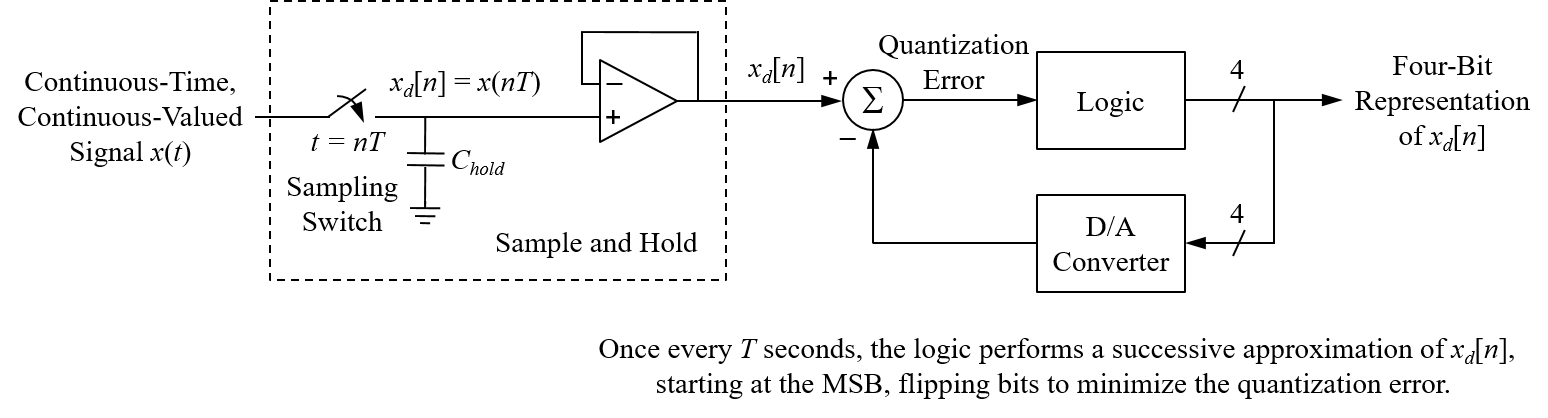
\includegraphics[width=\textwidth]{figs/ADC_EE102B.png}\\
		{\tiny \color{gray} Taken from the lecture notes of EE 102B by Prof. Joseph Kahn}
	\end{figure}
\end{block}

{\small More about ADCs in EE 315: Analog-Digital Interface Circuits.}

\end{frame}

%
\begin{frame}{Analog-to-digital conversion}

\begin{block}{In this class}
We'll model the ADC as an ideal continuous-to-discrete (C-to-D) time converter. 
\begin{center}
	\begin{tikzpicture}[->, >=stealth, shorten >= 0pt, draw=black!50, node distance=3cm, font=\sffamily]
	\tikzstyle{node}=[circle,fill=black,minimum size=2pt,inner sep=0pt]
	\tikzstyle{block}=[draw=black,rectangle,fill=none,minimum size=1.5cm, inner sep=0pt]
	\tikzstyle{annot} = []
	
	\node[node] (xc) {};
	\node[block, right of=xc, align=center, text width=2cm] (DSP) {C-to-D Converter};
	\coordinate[right of=DSP] (yc) {};
	
	\path (xc) edge (DSP);
	\path (DSP) edge (yc);
	
	\node[above = 0mm of xc, text width = 2cm, align=center] {$x_c(t)$};
	\node[below = 0mm of xc, text width = 2cm, align=center] {$X_c(j\Omega)$};
	\node[above = 0mm of yc, text width = 3cm, align=center] {$x[n] = x_c(nT)$}; 
	\node[below = 0mm of yc, text width = 2cm, align=center] {$X(e^{j\omega}), X(e^{j\Omega T})$};
	\end{tikzpicture}
\end{center}

\end{block}

\textbf{Notation:} \\
$X_c(j\Omega)$ denotes the Fourier transform of the continuous-time signal $x_c(t)$, where $\Omega$ is the continuous-time frequency.

$X(e^{j\omega})$ denotes the discrete-time Fourier transform of a discrete-time signal $x[n]$, where $\omega$ is the normalized frequency.  
\end{frame}

%
\begin{frame}{Continuous-to-discrete time conversion}

The C-to-D converter simply samples the continuous-time signal every $T$ seconds, where $T$ is the \textbf{sampling period}. 
\begin{center}
	\resizebox{0.5\linewidth}{!}{\begin{tikzpicture} 
\begin{axis}[
axis lines*=middle,
enlargelimits = true,
xmin=-1,
xmax=10,
ymin=-0.5,
ymax=3,
axis line style={->,>=stealth},
xlabel={$t$},
ylabel={$\textcolor{red}{x_c(t)}$},
%yticklabel style = {yshift=0.2cm},
every axis x label/.style={
    at={(ticklabel* cs:1)},
    anchor=north,
},
every axis y label/.style={
    at={(ticklabel* cs:1)},
    anchor=south,
},
xtick={0, 1, ..., 3},
%ytick={1},
%xtick={-3.14, -1, 1, 3.14},
xticklabels={0, $T$, $2T$, $3T$},
%xmajorgrids,
%ymajorgrids,
every outer y axis line/.append style={white!15!black},
every y tick label/.append style={font=\color{white!15!black}},
legend style={draw=white!15!black,fill=white,legend cell align=left}]

\pgfmathsetseed{103}
\addplot[ycomb, mark=*, line width=2pt, domain=0:10, samples=11, line width=1.5, mark options={scale=1,fill=white}] {sin(deg(x)) + 0.5*rand + 1.5};
\pgfmathsetseed{103}
\addplot[red, smooth, line width=2pt, domain=0:11, samples=12, line width=1.5] {sin(deg(x)) + 0.5*rand + 1.5};
\node (dots) at (axis cs: 4, -0.25) {$\ldots$};
\node at (axis cs: 6, 3) {$x[n] = \textcolor{red}{x_c(nT)}$};
\end{axis}
\end{tikzpicture}
}
\end{center}

\pause
\textbf{Question:} How are $x_c(t)$ and $x[n]$ related in the frequency domain? In other words, how to obtain the discrete-time Fourier transform $X(e^{j\omega})$ from the continuous-time Fourier transform $X_c(j\Omega)$?
\end{frame}

%
\begin{frame}{Continuous-to-discrete time conversion}
\textbf{Impulse sampling interpretation:}\\
We can think of the C-to-D converter as multiplication by an \textbf{impulse train}, followed by an impulse-to-sequence converter. 

This representation is purely for mathematical convenience.
\begin{center}
	\resizebox{\linewidth}{!}{\begin{tikzpicture}[->, >=stealth, shorten >= 0pt, draw=black!50, node distance=3cm, font=\sffamily]
	\tikzstyle{node}=[circle,fill=black,minimum size=2pt,inner sep=0pt]
	\tikzstyle{adder}=[draw=black, circle,minimum size=20pt,inner sep=0pt]
	\tikzstyle{block}=[draw=black,rectangle,fill=none,minimum size=1.5cm, inner sep=0pt]
	\tikzstyle{annot} = []
	
	\node[node] (xc) {};
	\node[adder, right=1.5cm of xc] (add) {\Large $\times$};
	\node[node, above=1cm of add] (st) {};
	\node[block, right of=add, text width=3cm, align=center] (b1) {\small Impulse train to discrete-time sequence};
	\coordinate[right of=b1] (yc) {};
	
	\path (xc) edge (add);
	\path (add) edge (b1);
	\path (b1) edge (yc);
	\path (st) edge (add);
	
	\node[text width = 4cm, align=center] at ($(st.center) + (15mm, 3mm)$) {$s(t) = \displaystyle\sum_{n=-\infty}^\infty\delta(t-nT)$};
	\node[above = 0mm of xc, text width = 2cm, align=center] {$x_c(t)$};
	\node[above = 0mm of yc, text width = 3cm, align=center] {$x[n] = x_c(nT)$}; 
	\node[text width = 3cm, align=center] at ($(add.east)!0.5!(b1.west) + (0,4mm)$) {$x_s(t)$}; 
	\draw[dashed] ($(add.west) - (0.25cm, 1.5cm)$) rectangle ($(b1.east) + (0.25cm, 2.5cm)$) {};
	\node at ($(add.west)!0.5!(b1.east) - (0, 1.2cm)$) {C-to-D converter};
\end{tikzpicture}}
\end{center}

\end{frame}

\begin{frame}{Impulse sampling example}
\vspace{-0.4cm}
\begin{center}
	\resizebox{0.9\linewidth}{!}{\begin{tikzpicture}
\onslide<1-|handout:1>{
\begin{axis}[
	name=plot1,
	axis lines*=middle,
	enlargelimits = true,
	clip=false,
	scale only axis,
	width=0.7\textwidth,
	height=0.1\textwidth,
	ymin=-2.5,
	ymax=2.5,
	xmin=-10,
	xmax=10,
	axis line style={->,>=stealth},
	xlabel={\small $t$},
	ylabel={\small $x_c(t)$},
	every axis x label/.style={
		at={(ticklabel* cs:1)},
		%xshift=0.2cm,
		anchor=north,
	},
	every axis y label/.style={
		at={(ticklabel* cs:0.8)},
		anchor=south,
		xshift=0.5cm,
	},
	xtick=\empty,
	ytick=\empty,
	%yticklabel={\small 0.25},
	%xtick={0, 3},
	%xticklabels={$0$, 3},
	every outer y axis line/.append style={white!15!black},
	every y tick label/.append style={font=\color{white!15!black}},
	legend style={draw=white!15!black,fill=white,legend cell align=left}]
	\addplot[smooth, line width=1pt, domain=-10:10, samples=51] {cos(deg(x/2)) - sin(deg(x)) + cos(deg(x/2)-45) - sin(deg(x/4)-154)};
\end{axis}
}
\onslide<2-|handout:1>{
\begin{axis}[
	name=plot2,
	at=(plot1.below south east), anchor=above north east,
	axis lines*=middle,
	enlargelimits = true,
	clip=false,
	scale only axis,
	width=0.7\textwidth,
	height=0.1\textwidth,
	ymin=0,
	ymax=1.5,
	xmin=-10,
	xmax=10,
	axis line style={->,>=stealth},
	xlabel={\small $t$},
	ylabel={\small $s(t)$},
	yticklabel style = {yshift=0.1cm},
	every axis x label/.style={
		at={(ticklabel* cs:1)},
		%xshift=0.2cm,
		anchor=north,
	},
	every axis y label/.style={
		at={(ticklabel* cs:0.8)},
		anchor=south,
		xshift=0.4cm,
	},
	ytick=\empty,
	xtick=\empty,
	every outer y axis line/.append style={white!15!black},
	every y tick label/.append style={font=\color{white!15!black}},
	legend style={draw=white!15!black,fill=white,legend cell align=left}]
	\addplot[dirac, mark=triangle*, fill=black, mark options={scale=0.75, fill=black}, line width=1pt, domain=-10:10, samples=21] {1};
\end{axis}
}
\onslide<3-|handout:1>{
\begin{axis}[
	name=plot3,
	at=(plot2.below south east), anchor=above north east,
	axis lines*=middle,
	enlargelimits = true,
	clip=false,
	scale only axis,
	width=0.7\textwidth,
	height=0.1\textwidth,
	ymin=-2.5,
	ymax=2.5,
	xmin=-10,
	xmax=10,
	axis line style={->,>=stealth},
	xlabel={\small $t$},
	ylabel={\small $x_s(t) = x_c(t)\cdot s(t)$},
	every axis x label/.style={
		at={(ticklabel* cs:1)},
		%xshift=0.2cm,
		anchor=north,
	},
	every axis y label/.style={
		at={(ticklabel* cs:0.8)},
		anchor=south,
		xshift=1.5cm,
	},
	xtick=\empty,
	ytick=\empty,
	every outer y axis line/.append style={white!15!black},
	every y tick label/.append style={font=\color{white!15!black}},
	legend style={draw=white!15!black,fill=white,legend cell align=left}]
	\addplot[dirac, mark=triangle*, fill=black, mark options={scale=0.75, fill=black}, line width=1pt, domain=-10:10, samples=21] {cos(deg(x/2)) - sin(deg(x)) + cos(deg(x/2)-45) - sin(deg(x/4)-154)};
	\addplot[smooth, black!10, line width=1pt, domain=-10:10, samples=51] {cos(deg(x/2)) - sin(deg(x)) + cos(deg(x/2)-45) - sin(deg(x/4)-154)};
\end{axis}
}

\onslide<4|handout:1>{
	\begin{axis}[
	name=plot4,
	at=(plot3.below south east), anchor=above north east,
	axis lines*=middle,
	enlargelimits = true,
	clip=false,
	scale only axis,
	width=0.7\textwidth,
	height=0.1\textwidth,
	ymin=-2.5,
	ymax=2.5,
	xmin=-10,
	xmax=10,
	axis line style={->,>=stealth},
	xlabel={\small $n$},
	ylabel={\small $x[n]$},
	every axis x label/.style={
		at={(ticklabel* cs:1)},
		%xshift=0.2cm,
		anchor=north,
	},
	every axis y label/.style={
		at={(ticklabel* cs:0.8)},
		anchor=south,
		xshift=0.4cm,
	},
	xtick=\empty,
	ytick=\empty,
	every outer y axis line/.append style={white!15!black},
	every y tick label/.append style={font=\color{white!15!black}},
	legend style={draw=white!15!black,fill=white,legend cell align=left}]
	\addplot[ycomb, mark=*, fill=black, mark options={scale=0.75, fill=white}, line width=1pt, domain=-10:10, samples=21] {cos(deg(x/2)) - sin(deg(x)) + cos(deg(x/2)-45) - sin(deg(x/4)-154)};
	\addplot[smooth, black!10, line width=1pt, domain=-10:10, samples=51] {cos(deg(x/2)) - sin(deg(x)) + cos(deg(x/2)-45) - sin(deg(x/4)-154)};
	\end{axis}
}
\end{tikzpicture}
}
\end{center}
\end{frame}

\begin{frame}{Continuous-to-discrete time conversion}
\textbf{Question:} How to obtain the discrete-time Fourier transform $X(e^{j\omega})$ from the continuous-time Fourier transform $X_c(j\Omega)$?
\begin{center}
	\resizebox{\linewidth}{!}{\begin{tikzpicture}[->, >=stealth, shorten >= 0pt, draw=black!50, node distance=3cm, font=\sffamily]
	\tikzstyle{node}=[circle,fill=black,minimum size=2pt,inner sep=0pt]
	\tikzstyle{adder}=[draw=black, circle,minimum size=20pt,inner sep=0pt]
	\tikzstyle{block}=[draw=black,rectangle,fill=none,minimum size=1.5cm, inner sep=0pt]
	\tikzstyle{annot} = []
	
	\node[node] (xc) {};
	\node[adder, right=1.5cm of xc] (add) {\Large $\times$};
	\node[node, above=1cm of add] (st) {};
	\node[block, right of=add, text width=3cm, align=center] (b1) {\small Impulse train to discrete-time sequence};
	\coordinate[right of=b1] (yc) {};
	
	\path (xc) edge (add);
	\path (add) edge (b1);
	\path (b1) edge (yc);
	\path (st) edge (add);
	
	\node[text width = 4cm, align=center] at ($(st.center) + (15mm, 3mm)$) {$s(t) = \displaystyle\sum_{n=-\infty}^\infty\delta(t-nT)$};
	\node[above = 0mm of xc, text width = 2cm, align=center] {$x_c(t)$};
	\node[above = 0mm of yc, text width = 3cm, align=center] {$x[n] = x_c(nT)$}; 
	\node[text width = 3cm, align=center] at ($(add.east)!0.5!(b1.west) + (0,4mm)$) {$x_s(t)$}; 
	\draw[dashed] ($(add.west) - (0.25cm, 1.5cm)$) rectangle ($(b1.east) + (0.25cm, 2.5cm)$) {};
	\node at ($(add.west)!0.5!(b1.east) - (0, 1.2cm)$) {C-to-D converter};
\end{tikzpicture}}
\end{center}

We'll calculate the continuous-time (CT) Fourier transform of $x_s(t)$ in two different ways. First, we'll calculate $X_s(j\Omega) = \frac{1}{2\pi}X_c(j\Omega)\ast S(j\Omega)$. Then, we'll calculate $X_s(j\Omega) = \mathcal{F}\{x_s(t)\}$. We'll use these two equations of $X_s(j\Omega)$ to obtain an equation for $X(e^{j\omega})$, the DTFT of $x[n]$.

\end{frame}

%
\begin{frame}

Starting with $X_s(j\Omega) = \frac{1}{2\pi}X_c(j\Omega)\ast S(j\Omega)$, recall that the Fourier transform of the impulse train is given by
\begin{equation*}
s(t) = \sum_{n=-\infty}^\infty \delta(t-nT) \Longleftrightarrow S(j\Omega) = \sum_{k=-\infty}^\infty \frac{2\pi}{T}\delta\Big(\Omega-k\frac{2\pi}{T}\Big)
\end{equation*}

Now we can calculate $X_s(j\Omega)$:
\begin{align} \nonumber
X_s(j\Omega) &= \frac{1}{2\pi}X_c(j\Omega) \ast S(j\Omega) \\ \nonumber
X_s(j\Omega) &= \frac{1}{2\pi}X_c(j\Omega) \ast \bigg(\sum_{k=-\infty}^\infty\frac{2\pi}{T}\delta\Big(\Omega-k\frac{2\pi}{T}\Big)\bigg) \\ 
&\tikz[baseline]{
	\node[fill=blue!20,anchor=base] (t1) {$X_s(j\Omega) = \displaystyle\sum_{k=-\infty}^\infty\frac{1}{T}X_c\Big(j\Big(\Omega-k\frac{2\pi}{T}\Big)\Big)$};} \label{eq:Xs1}
\end{align}

Note that $X_s(j\Omega)$ is equal to $X_c(j\Omega)$ scaled by $1/T$ and repeated every $2\pi/T$, which we define as the \textbf{sampling frequency} $\Omega_s \equiv  2\pi/T$
\end{frame}

%
\begin{frame}
Now let's calculate $X_s(j\Omega) = \mathcal{F}\{x_s(t)\}$, where $x_s(t) = x_c(t)\cdot s(t)$:
\begin{align} \nonumber
X_s(j\Omega) &= \mathcal{F}\{x_c(t)\cdot s(t)\} = \mathcal{F}\bigg\lbrace \sum_{n=-\infty}^{\infty} x_c(nT)\delta(t-nT) \bigg\rbrace \\ \nonumber
&= \mathcal{F}\bigg\lbrace \sum_{n=-\infty}^{\infty} x[n]\delta(t-nT) \bigg\rbrace \\ \nonumber
&= \int_{-\infty}^{\infty}\sum_{n=-\infty}^{\infty} x[n]\delta(t-nT)e^{-j\Omega t}dt \tag{CT Fourier transform} \\ \nonumber
&= \sum_{n=-\infty}^{\infty} x[n]\int_{-\infty}^{\infty}\delta(t-nT)e^{-j\Omega t}dt \\ \nonumber
&= \sum_{n=-\infty}^{\infty} x[n]e^{-jn\Omega T} \tag{recall: $X(e^{j\omega}) \equiv \sum_{n=-\infty}^{\infty} x[n]e^{-jn\omega}$} \\
&\tikz[baseline]{
	\node[fill=blue!20,anchor=base] (t1) {$X_s(j\Omega) = X(e^{j\omega})\Big|_{\omega=\Omega T}$};} \label{eq:Xs2}
\end{align}

$X_s(j\Omega)$ is equal to $X(e^{j\omega})$ evaluated at $\omega = \Omega T$, or equivalently $X(e^{j\omega})$  is equal to $X_s(j\Omega)$ evaluated at $\Omega = \omega/T$.
\end{frame}

%
\begin{frame}
Substituting \eqref{eq:Xs1} in \eqref{eq:Xs2}:
\begin{equation*}
X(e^{j\Omega T}) = \frac{1}{T}\sum_{k=-\infty}^{\infty} X_c\Big(j\Big(\Omega - k\frac{2\pi}{T}\Big)\Big),
\end{equation*}
where we used the relation $\omega = \Omega T$.

\begin{itemize}
	\item $T$ is the \textbf{sampling period}, and $\Omega_s = \frac{2\pi}{T}$ is the \textbf{sampling frequency}
	\item This equation shows that in discrete time ($\omega = \Omega T$) replicas of the original spectrum appear with period $2\pi$
\end{itemize}

\end{frame}

\begin{frame}{Graphically}
\vspace{-0.4cm}
\begin{center}
	\resizebox{0.85\linewidth}{!}{\begin{tikzpicture}
\onslide<1-|handout:1>{
\begin{axis}[
	name=plot1,
	axis lines*=middle,
	enlargelimits = true,
	clip=false,
	scale only axis,
	width=0.7\textwidth,
	height=0.1\textwidth,
	ymin=0,
	ymax=3,
	xmin=-10,
	xmax=10,
	axis line style={->,>=stealth},
	xlabel={\small $\Omega$},
	ylabel={\small $X_c(j\Omega)$},
	every axis x label/.style={
		at={(ticklabel* cs:1)},
		%xshift=0.2cm,
		anchor=north,
	},
	every axis y label/.style={
		at={(ticklabel* cs:0.8)},
		anchor=south,
		xshift=0.6cm,
	},
	ytick=2,
	xtick=\empty,
	yticklabel={\small 1},
	xtick={-2.5, 2.5},
	xticklabels={\small $-\Omega_N$, \small $\Omega_N$},
	every outer y axis line/.append style={white!15!black},
	every y tick label/.append style={font=\color{white!15!black}},
	legend style={draw=white!15!black,fill=white,legend cell align=left}]
	\addplot[solid, line width=1pt] coordinates {(0, 2) (2.5, 0) (0, 0)};
	\addplot[solid, line width=1pt, fill=blue!50] coordinates {(0, 2) (-2.5, 0) (0, 0)};
\end{axis}
}
\onslide<2-|handout:1>{
\begin{axis}[
	name=plot2,
	at=(plot1.below south east), anchor=above north east,
	axis lines*=middle,
	enlargelimits = true,
	clip=false,
	scale only axis,
	width=0.7\textwidth,
	height=0.1\textwidth,
	ymin=0,
	ymax=1.5,
	xmin=-10,
	xmax=10,
	axis line style={->,>=stealth},
	xlabel={\small $\Omega$},
	ylabel={\small $S(j\Omega)$},
	yticklabel style = {yshift=0.1cm},
	every axis x label/.style={
		at={(ticklabel* cs:1)},
		%xshift=0.2cm,
		anchor=north,
	},
	every axis y label/.style={
		at={(ticklabel* cs:0.8)},
		anchor=south,
		xshift=0.5cm,
	},
	ytick={1},
	yticklabels={\small $\frac{2\pi}{T}$},
	xtick={-6, 0, 6},
	xticklabels={\small $-\Omega_s$, \small 0, \small $\Omega_s$}, 
	every outer y axis line/.append style={white!15!black},
	every y tick label/.append style={font=\color{white!15!black}},
	legend style={draw=white!15!black,fill=white,legend cell align=left}]
	\addplot[dirac, mark=triangle*, fill=black, mark options={scale=0.75, fill=black}, line width=1pt, domain=-6:6, samples=3] {1};
\end{axis}
}
\onslide<3-|handout:1>{
\begin{axis}[
	name=plot3,
	at=(plot2.below south east), anchor=above north east,
	axis lines*=middle,
	enlargelimits = true,
	clip=false,
	scale only axis,
	width=0.7\textwidth,
	height=0.1\textwidth,
	ymin=0,
	ymax=3,
	xmin=-10,
	xmax=10,
	axis line style={->,>=stealth},
	xlabel={\small $\Omega$},
	ylabel={\small $X_s(j\Omega) = \frac{1}{2\pi}X_c(j\Omega)\ast S(j\Omega)$},
	every axis x label/.style={
		at={(ticklabel* cs:1)},
		%xshift=0.2cm,
		anchor=north,
	},
	every axis y label/.style={
		at={(ticklabel* cs:0.8)},
		anchor=south,
		xshift=2.2cm,
	},
	xtick=\empty,
	ytick=2,
	yticklabels={\small $1/T$},
	xtick={-6, -2.5, 0, 2.5, 6},
	xticklabels={\small $-\Omega_s$, \small $-\Omega_N$, \small 0, \small $\Omega_N$, \small $\Omega_s$}, 
	every outer y axis line/.append style={white!15!black},
	every y tick label/.append style={font=\color{white!15!black}},
	legend style={draw=white!15!black,fill=white,legend cell align=left}]
	\addplot[solid, line width=1pt] coordinates {(0, 2) (2.5, 0) (0, 0)};
	\addplot[solid, line width=1pt, fill=blue!50] coordinates {(0, 2) (-2.5, 0) (0, 0)};
	\addplot[solid, line width=1pt] coordinates {(6, 2) (8.5, 0) (6, 0)};
	\addplot[solid, line width=1pt, fill=blue!50] coordinates {(6, 2) (3.5, 0) (6, 0)};
	\addplot[solid, line width=1pt] coordinates {(-6, 2) (-3.5, 0) (-6, 0)};
	\addplot[solid, line width=1pt, fill=blue!50] coordinates {(-6, 2) (-8.5, 0) (-6, 0)};
	
\end{axis}
}

\onslide<4|handout:1>{
\begin{axis}[
name=plot4,
at=(plot3.below south east), anchor=above north east,
axis lines*=middle,
enlargelimits = true,
clip=false,
scale only axis,
width=0.7\textwidth,
height=0.1\textwidth,
ymin=0,
ymax=3,
xmin=-10,
xmax=10,
axis line style={->,>=stealth},
xlabel={\small $\omega=\Omega T$},
ylabel={\small $X(e^{j\omega}) = X(j\Omega)$},
every axis x label/.style={
	at={(ticklabel* cs:1)},
	%xshift=0.2cm,
	anchor=north,
},
every axis y label/.style={
	at={(ticklabel* cs:0.8)},
	anchor=south,
	xshift=1.2cm,
},
xtick=\empty,
ytick=2,
yticklabels={\small $1/T$},
xtick={-6, -2.5, 0, 2.5, 6},
xticklabels={\small $-2\pi$, \small $-\Omega_NT$, \small 0, \small $\Omega_NT$, \small $2\pi$}, 
every outer y axis line/.append style={white!15!black},
every y tick label/.append style={font=\color{white!15!black}},
legend style={draw=white!15!black,fill=white,legend cell align=left}]
\addplot[solid, line width=1pt] coordinates {(0, 2) (2.5, 0) (0, 0)};
\addplot[solid, line width=1pt, fill=blue!50] coordinates {(0, 2) (-2.5, 0) (0, 0)};
\addplot[solid, line width=1pt] coordinates {(6, 2) (8.5, 0) (6, 0)};
\addplot[solid, line width=1pt, fill=blue!50] coordinates {(6, 2) (3.5, 0) (6, 0)};
\addplot[solid, line width=1pt] coordinates {(-6, 2) (-3.5, 0) (-6, 0)};
\addplot[solid, line width=1pt, fill=blue!50] coordinates {(-6, 2) (-8.5, 0) (-6, 0)};

\end{axis}
}
\end{tikzpicture}
}
\end{center}
\vspace{-0.4cm}
\onslide<4|handout:1>{Replicas of the original spectrum appear with period $2\pi$}
\end{frame}

\begin{frame}{Oversampling}
\begin{itemize}
	\item A signal is \textbf{band limited} if $X_c(j\Omega) = 0$ for $|\Omega| > \Omega_N$. In this case, the signal has maximum frequency $\Omega_N$ and \textbf{bandwidth} $2\Omega_N$
	\item Sampling at $\Omega_s > 2\Omega_N$ is called \textbf{oversampling}
	\item We can define an \textbf{oversampling ratio} $r_{os}\equiv \frac{\Omega_s}{2\Omega_N}$
	\item Note that if $\Omega_s > 2\Omega_N$ ($r_{os} > 1$), there'll be a gap between the spectrum replicas
\end{itemize}

\begin{center}
	\resizebox{0.8\linewidth}{!}{\PlotSampledSpectrum{figs/oversampling_example.tex}{10.0}{5.0}{$\Omega_s > 2\Omega_N$}}
\end{center}
\end{frame}

\begin{frame}{Nyquist sampling}
\begin{itemize}
	\item Sampling at $\Omega_s = 2\Omega_N$ ($r_{os} = 1$) is called \textbf{Nyquist sampling}
	\item Note that if $\Omega_s$ is any smaller than $2\Omega_N$, there will be overlapping of the spectrum replicas
	
\begin{center}
		\resizebox{0.9\linewidth}{!}{\PlotSampledSpectrum{figs/oversampling_example.tex}{5}{2.5}{$\Omega_s = 2\Omega_N$}}
\end{center}
\end{itemize}
\end{frame}


\begin{frame}{Undersampling}
\begin{itemize}
	\item Undersampling occurs when $\Omega_s < 2\Omega_N$ ($r_{os} < 1$)
	\item In this case, the spectrum replicas overlap
	\item The overlapping causes \textbf{aliasing distortion}
\end{itemize}

\begin{center}
	\resizebox{0.9\linewidth}{!}{\def\fs{3.5}
\def\fmax{1.75}
\begin{tikzpicture}
\begin{axis}[
	name=plot1,
	axis lines*=middle,
	enlargelimits = true,
	clip=false,
	scale only axis,
	width=0.8\textwidth,
	height=0.2\textwidth,
	ymin=0,
	ymax=3,
	xmin=-6,
	xmax=6,
	axis line style={->,>=stealth},
	xlabel={\small $\Omega$},
	ylabel={\small $X_c(j\Omega)$},
	every axis x label/.style={
		at={(ticklabel* cs:1)},
		%xshift=0.2cm,
		anchor=north,
	},
	every axis y label/.style={
		at={(ticklabel* cs:0.8)},
		anchor=south,
		xshift=0.6cm,
	},
	ytick=2,
	xtick=\empty,
	yticklabel={\small 1},
	xtick={-2.5, 2.5},
	xticklabels={\small $-\Omega_N$, \small $\Omega_N$},
	every outer y axis line/.append style={white!15!black},
	every x tick label/.append style={font=\color{white!15!black}},
	legend style={draw=white!15!black,fill=white,legend cell align=left}]
	\addplot[solid, line width=1pt] coordinates {(0, 2) (2.5, 0) (0, 0)};
	\addplot[solid, line width=1pt, fill=blue!50] coordinates {(0, 2) (-2.5, 0) (0, 0)};
\end{axis}

\begin{axis}[
	name=plot2,
	at=(plot1.below south east), anchor=above north east,
	axis lines*=middle,
	enlargelimits = true,
	axis on top=true,
	clip=true,
	scale only axis,
	width=0.8\textwidth,
	height=0.2\textwidth,
	ymin=0,
	ymax=3,
	xmin=-6,
	xmax=6,
	axis line style={->,>=stealth},
	xlabel={\small $\omega=\Omega T$},
	ylabel={\small $X(e^{j\omega})$},
	every axis x label/.style={
		at={(ticklabel* cs:1)},
		%xshift=0.2cm,
		anchor=north,
	},
	every axis y label/.style={
		at={(ticklabel* cs:0.8)},
		anchor=south,
		xshift=0.5cm,
	},
	xtick={-\fs, -\fmax, \fmax, \fs},
	xticklabels={\small $-2\pi$, \small $-\pi$, \small $\pi$, \small $2\pi$},
	ytick=2,
	yticklabels={\small $1/T$},
	every outer y axis line/.append style={white!15!black},
	every y tick label/.append style={font=\color{white!15!black}},
	legend style={draw=white!15!black,fill=white,legend cell align=left}]
	\addplot[solid, line width=0pt] coordinates {(\fs, 2) (\fs+2.5, 0) (\fs, 0)};
	\addplot[solid, line width=0pt, fill=blue!50] coordinates {(\fs, 2) (\fs-2.5, 0) (\fs, 0)};
	\addplot[name path=pos, solid, line width=1pt] coordinates {(\fs-2.5, 0) (\fs, 2)};
	
	\addplot[solid, line width=0pt] coordinates {(0, 2) (2.5, 0) (0, 0)};
	\addplot[solid, line width=0pt, fill=blue!50] coordinates {(0, 2) (-2.5, 0) (0, 0)};
	\addplot[name path=zer1, solid, line width=1pt] coordinates {(0, 2) (2.5, 0)};
	\addplot[name path=zer2, solid, line width=1pt] coordinates {(0, 2) (-2.5, 0)};
	
	\addplot[solid, line width=0pt] coordinates {(-\fs, 2) (-\fs+2.5, 0) (-\fs, 0)};
	\addplot[solid, line width=0pt, fill=blue!50] coordinates {(-\fs, 2) (-\fs-2.5, 0) (-\fs, 0)};
	\addplot[name path=neg, solid, line width=1pt] coordinates {(-\fs+2.5, 0) (-\fs, 2) };
	
	%\fill[red!70, intersection segments={of=pos and zer1}];
	%\fill[red!70, intersection segments={of=neg and zer2}];	
	
	%\addplot[solid, line width=1pt] coordinates {(\fs, 2) (\fs+1, 1.2) (\fs+2.5, 1.2)};
	\addplot[fill=red!50, red!50, line width=0pt] coordinates {(-\fs-2.5, 1.2) (-\fs-2.5, 0) (-\fs-1, 0) (-\fs-1, 1.2) (-\fs-2.5, 1.2)};
	\addplot[fill=red!50, red!50, line width=0pt] coordinates {(-2.5, 1.2) (-2.5, 0) (-1, 0) (-1, 1.2) (-2.5, 1.2)};
	\addplot[fill=red!50, red!50, line width=0pt] coordinates {(\fs-2.5, 1.2) (\fs-2.5, 0) (\fs-1, 0) (\fs-1, 1.2) (\fs-2.5, 1.2)};
	\addplot[fill=red!50, red!50, line width=0pt] coordinates {(\fs+2.5, 1.2) (\fs+2.5, 0) (\fs+1, 0) (\fs+1, 1.2) (\fs+2.5, 1.2)};
	\addplot[solid, line width=1.5pt] coordinates {(-\fs-2.5, 1.2) (-\fs-1, 1.2) (-\fs, 2) (-\fs+1, 1.2) (-\fs+2.5, 1.2) (0, 2) (1, 1.2) (2.5, 1.2) (\fs, 2) (\fs+1, 1.2) (\fs+2.5, 1.2)};

	\addplot[black!50, dashed, line width=1pt] coordinates {(-\fs-2.5, 0) (-\fs-1, 1.2)};
	\addplot[black!50, dashed, line width=1pt] coordinates {(-\fs-2.5, 1.2) (-\fs-1, 0)};
	
	\addplot[black!50, dashed, line width=1pt] coordinates {(-2.5, 0) (-1, 1.2)};
	\addplot[black!50, dashed, line width=1pt] coordinates {(-2.5, 1.2) (-1, 0)};
	
	\addplot[black!50, dashed, line width=1pt] coordinates {(2.5, 0) (1, 1.2)};
	\addplot[black!50, dashed, line width=1pt] coordinates {(2.5, 1.2) (1, 0)};
	
	\addplot[black!50, dashed, line width=1pt] coordinates {(\fs-2.5, 0) (\fs-1, 1.2)};
	\addplot[black!50, dashed, line width=1pt] coordinates {(\fs-2.5, 1.2) (\fs-1, 0)};

	\addplot[black!50, dashed, line width=1pt] coordinates {(\fs+2.5, 0) (\fs+1, 1.2)};
	\addplot[black!50, dashed, line width=1pt] coordinates {(\fs+2.5, 1.2) (\fs+1, 0)};
	
\end{axis}
\end{tikzpicture}
}
\end{center}
The regions in red are the regions where the spectrum replicas overlap
\end{frame}

\begin{frame}{Aliasing: time domain}
\only<1|handout:0>{A sinusoidal signal with frequency $\Omega_N = 1.5\pi$}
\only<2|handout:0>{Samples taken at frequency $\Omega_s = 2\pi$. Therefore, $r_{os} = \frac{\Omega_s}{2\Omega_N} = \frac{2}{3} < 1$}
\only<3|handout:1>{Samples taken at frequency $\Omega_s = 2\pi$ form an {\color{red} \textbf{alias signal}} of frequency $0.5\pi$, but {\color{gray} \textbf{original signal}} had frequency $1.5\pi$}
\begin{center}
	\resizebox{0.7\linewidth}{!}{\begin{tikzpicture} 
\begin{axis}[
axis lines*=middle,
enlargelimits = true,
ymin=-1.2,
ymax=1.2,
xmin=0,
xmax=10,
axis line style={->,>=stealth},
%xlabel={\Large $n$},
%ylabel={\Large $x[n]$},
yticklabel style = {yshift=0.2cm},
xticklabel style = {yshift=-0.1cm},
every axis x label/.style={
    at={(ticklabel* cs:1)},
    anchor=north,
},
every axis y label/.style={
    at={(ticklabel* cs:1)},
    anchor=south,
},
%xtick=\empty,
ytick=\empty,
xtick=\empty,
every outer y axis line/.append style={white!15!black},
every y tick label/.append style={font=\color{white!15!black}},
legend style={draw=white!15!black,fill=white,legend cell align=left}]

\only<1|handout:1>{
\addplot[smooth, line width=1.5pt, domain=0:10, samples=101] {cos(deg(2*pi*0.75*x))};
}

\only<2-|handout:1>{
\addplot[smooth, black!50, line width=1.5pt, domain=0:10, samples=101] {cos(deg(2*pi*0.75*x))};
\addplot[ycomb, mark=*, fill=white, mark options={scale=1.5, fill=white}, line width=1.5pt, domain=0:10, samples=11] {cos(deg(2*pi*0.75*x))};
}

\only<3-|handout:1>{
\addplot[smooth, red, line width=1.5pt, domain=0:10, samples=51] {cos(deg(2*pi*0.25*x))};
}

\end{axis}
\end{tikzpicture}
}
\end{center}
\end{frame}

\begin{frame}{Aliasing: frequency domain}
Same example, but now in the frequency domain
\begin{center}
	\resizebox{0.9\linewidth}{!}{\begin{tikzpicture}
\begin{axis}[
	name=plot1,
	axis lines*=middle,
	enlargelimits = true,
	clip=false,
	scale only axis,
	width=0.8\textwidth,
	height=0.2\textwidth,
	ymin=0,
	ymax=1,
	xmin=-3.2,
	xmax=3.2,
	axis line style={->,>=stealth},
	xlabel={\small $\Omega$},
	ylabel={\small $X(j\omega)$},
	every axis x label/.style={
		at={(ticklabel* cs:1)},
		%xshift=0.2cm,
		anchor=north,
	},
	every axis y label/.style={
		at={(ticklabel* cs:0.8)},
		anchor=south,
		xshift=0.6cm,
	},
	ytick=\empty,
	xtick={-1.5, 1.5},
	xticklabels={\small $-1.5\pi$, \small $1.5\pi$},
	every outer y axis line/.append style={white!15!black},
	every x tick label/.append style={font=\color{white!15!black}},
	legend style={draw=white!15!black,fill=white,legend cell align=left}]
	\addplot[dirac, mark=triangle*, fill=black, mark options={scale=0.75, fill=black}, line width=1pt] coordinates {(-1.5, 0.5) (1.5, 0.5)};
\end{axis}

\begin{axis}[
	name=plot2,
	at=(plot1.below south east), anchor=above north east,
	axis lines*=middle,
	enlargelimits = true,
	axis on top=true,
	clip=true,
	scale only axis,
	width=0.8\textwidth,
	height=0.2\textwidth,
	ymin=0,
	ymax=1,
	xmin=-3.2,
	xmax=3.2,
	axis line style={->,>=stealth},
	xlabel={\small $\omega=\Omega T$},
	ylabel={\small $X(e^{j\omega})$},
	every axis x label/.style={
		at={(ticklabel* cs:1)},
		%xshift=0.2cm,
		anchor=north,
	},
	every axis y label/.style={
		at={(ticklabel* cs:0.8)},
		anchor=south,
		xshift=0.6cm,
	},
	xtick={-2, -1, 0.5, 1, 1.5, 2},
	xticklabels={\scriptsize $-2\pi$, \scriptsize $-\pi$, \scriptsize $0.5\pi$, \scriptsize $\pi$, \scriptsize $1.5\pi$, \scriptsize $2\pi$},
	ytick=\empty,
	every outer y axis line/.append style={white!15!black},
	every y tick label/.append style={font=\color{white!15!black}},
	legend style={draw=white!15!black,fill=white,legend cell align=left}]
	\addplot[ycomb, mark=*, fill=black, mark options={scale=0.75, fill=white}, line width=1pt] coordinates {(-1.5, 0.5) (1.5, 0.5)};
	\only<2-|handout:1>{
	\addplot[ycomb, blue2, mark=*, fill=black, mark options={scale=0.75, fill=white}, line width=1pt] coordinates {(0.5, 0.5) (3.5, 0.5)};}
	\only<3-|handout:1>{
	\addplot[ycomb, red2, mark=*, fill=black, mark options={scale=0.75, fill=white}, line width=1pt] coordinates {(-0.5, 0.5) (-3.5, 0.5)};}
	
\end{axis}
\end{tikzpicture}
}
\end{center}

\onslide<3-|handout:1>{
Blue components correspond to spectrum replica centered at $2\pi$, while red components correspond to spectrum replica centered at $-2\pi$.

The final spectrum corresponds to $\cos(0.5\pi n)$
}

\end{frame}

%
\begin{frame}{Aliasing examples}

Cameras and our own visual system are sampling devices with a certain sampling frequency. Therefore, we can \textit{see} aliasing.

\begin{block}{Examples}
	\begin{itemize}
		\item This \href{https://www.youtube.com/watch?v=R-IVw8OKjvQ}{video}. 		
		The blades of the helicopter are spinning at the same frequency of the camera shutter
		\item Wheels of the car that appear to spin backwards
		\item Stroboscopic effect (search videos of this)
	\end{itemize}
\end{block}
\end{frame}

%
\begin{frame}{Sampling random signals}

The same theory applies to random signals. Specifically, we we'll apply the same results to the autocorrelation function and PSD of random signals

Autocorrelation function of a continuous-time WSS process and its PSD:
\begin{equation*}
\phi_{x_cx_c}(\tau) = \E(x_c(t+\tau)x_c^*(t)) \Longleftrightarrow \Phi_{x_cx_c}(j\Omega)
\end{equation*}

If we sample the random signal with sampling period $T = 2\pi/\Omega_s$, we obtain $x[n] = x_c(nT)$. Calculating the autocorrelation function of $x[n]$:
\begin{align*}
\phi_{xx}[m] &= \E(x[n+m]x^*[n]) = \E(x_c((n+m)T)x_c^*(nT)) \\
&= \phi_{x_cx_c}(mT) \tag{the autocorrelation is sampled}
\end{align*}

And for the PSD:
\begin{align*}
\Phi_{xx}(e^{j\Omega T}) &= \mathcal{F}(\phi_{xx}[m]) = \sum_{m=-\infty}^{\infty}\phi_{xx}[m]e^{-j\Omega T} \\
&= \frac{1}{T}\sum_{k=-\infty}^{\infty}\Phi_{x_cx_c}(j(\Omega-k\Omega_s)) \tag{the PSD is replicated with period $\Omega_s$}
\end{align*}

\end{frame}


\section{Reconstruction}
\begin{frame}{Digital processing of analog signals}
\begin{block}{Typical system}
	\vspace{-0.7cm}
	\begin{center}
		\resizebox{\linewidth}{!}{\def\layersep{1.5cm}
\def\outsep{0.7cm}
\def\dy{1.25}

\begin{tikzpicture}[->, >=stealth, shorten >= 0pt, draw=black!50, node distance=\layersep, font=\sffamily]
    \tikzstyle{node}=[circle,fill=black,minimum size=2pt,inner sep=0pt]
    \tikzstyle{block}=[draw=black,rectangle,fill=none,minimum size=1.5cm, inner sep=0pt]
    \tikzstyle{annot} = []

	\node[node] (xc) at (0, -\dy cm) {};
    \node[block] (ADC) at (1*\layersep, -\dy cm) {ADC};
    \node[block, text width = 2.5cm, align= center] (DSP) at (3*\layersep, -\dy cm) {Digital Signal Processor};
    \node[block] (DAC) at (5*\layersep, -\dy cm) {DAC};
	\coordinate (yc) at (6*\layersep, -\dy cm) {};
	
	\coordinate (mid1) at ($(ADC.east)!0.5!(DSP.west)$) {};
	\coordinate (mid2) at ($(DSP.east)!0.5!(DAC.west)$) {};
		
    \path (xc) edge (ADC);
    \path (ADC) edge (DSP);
    \path (DSP) edge (DAC);
    \path (DAC) edge (yc);
    
    \node[above = 0.5mm of mid1] {$x[n]$};
    \node[above = 0.5mm of mid2] {$y[n]$};
    \node[left = 0mm of xc, text width = 1cm, align=center] {$x_c(t)$};
    \node[right = 0mm of yc, text width = 1cm, align=center] {$y_c(t)$}; 
    

\end{tikzpicture}}
	\end{center}
\end{block}
\vspace{-0.5cm}
\begin{block}{Analog-to-digital converter (ADC)}
	\begin{itemize}
		\item Performs filtering, sampling, and quantization
		\item Sampling rate may be of tens of kHz (audio processing), or it may be of tens of GHz (optical communications)
	\end{itemize}
\end{block}
\vspace{-0.3cm}
\begin{block}{Digital signal processor}
	\begin{itemize} \itemsep 0pt
		\item Performs some operation e.g., filtering, FFT, etc
		\item May be implemented on PCs with 64-bit floating-point precision, or on ASICs with limited arithmetic precision (e.g., 6 bits).
	\end{itemize}
\end{block}
\vspace{-0.3cm}
\begin{block}{\textbf{Digital-to-analog converter (DAC)}}
	\begin{itemize}
		\item Performs quantization and reconstruction (filtering)
		\item Sampling rate could be similar to ADC
	\end{itemize}
\end{block}
\end{frame}

\begin{frame}{Digital-to-analog conversion}

\begin{block}{In practice}
	Example of digital-to-analog converter (DAC)
	\begin{figure}
		\centering
		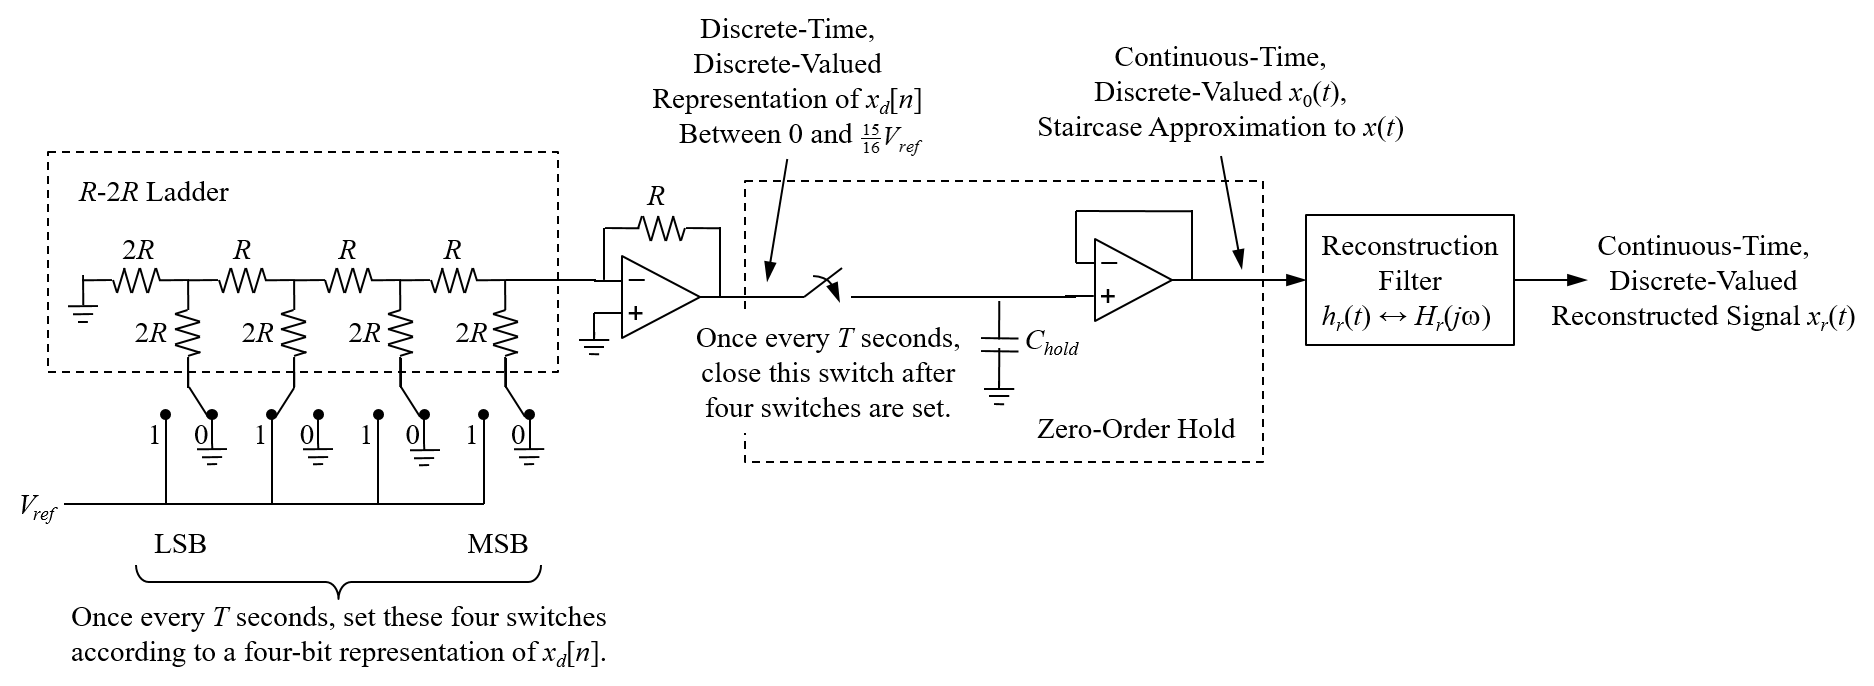
\includegraphics[width=\textwidth]{figs/DAC_EE102B.png}\\
		{\tiny \color{gray} Taken from the lecture notes of EE 102B by Prof. Joseph Kahn}
	\end{figure}
\end{block}

\end{frame}


\begin{frame}{Digital-to-analog conversion}

\begin{block}{In this class}
We'll model the ADC as an ideal discrete-to-continuous (D-to-C) time converter. 
\begin{center}
	\begin{tikzpicture}[->, >=stealth, shorten >= 0pt, draw=black!50, node distance=3cm, font=\sffamily]
	\tikzstyle{node}=[circle,fill=black,minimum size=2pt,inner sep=0pt]
	\tikzstyle{block}=[draw=black,rectangle,fill=none,minimum size=1.5cm, inner sep=0pt]
	\tikzstyle{annot} = []
	
	\node[node] (xc) {};
	\node[block, right of=xc, align=center, text width=2cm] (DSP) {D-to-C Converter};
	\coordinate[right of=DSP] (yc) {};
	
	\path (xc) edge (DSP);
	\path (DSP) edge (yc);
	
	\node[above = 0mm of xc, text width = 2cm, align=center] {$x[n]$};
	\node[below = 0mm of xc, text width = 2cm, align=center] {$X(e^{j\omega}), X(e^{j\Omega T})$};
	\node[above = 0mm of yc, text width = 3cm, align=center] {$x_c(t)$}; 
	\node[below = 0mm of yc, text width = 2cm, align=center] {$X(j\Omega)$};
	\end{tikzpicture}
\end{center}
\end{block}
In essence, a D-to-C converter performs \textbf{interpolation}.
\end{frame}

\begin{frame}{Discrete-to-continuous time conversion}
For mathematical convenience we can model the D-to-C as
\begin{center}
	\begin{tikzpicture}[->, >=stealth, shorten >= 0pt, draw=black!50, node distance=4cm, font=\sffamily]
		\tikzstyle{node}=[circle,fill=black,minimum size=2pt,inner sep=0pt]
		\tikzstyle{block}=[draw=black,rectangle,fill=none,minimum size=1.5cm, inner sep=0pt]
		\tikzstyle{annot} = []
		
		\node[node] (xc) {};
		\node[block, right=1.5cm of xc, text width=3cm, align=center] (b1) {\small Discrete-time sequence to impulse train};
		\node[block, right=0.5cm of b1, text width=2.5cm, align=center] (b2) {\small Lowpass filter $h_r(t) \leftrightarrow H_r(j\Omega)$};
		\coordinate[right=1.5cm of b2.east] (yc) {};
		
		\path (xc) edge (b1);
		\path (b1) edge (b2);
		\path (b2) edge (yc);
				
		\node[above = 0mm of xc, text width = 2cm, align=center] {$x[n]$};
		\node[above = 0mm of yc, text width = 3cm, align=center] {$x_r(t)$}; 
		\draw[dashed] ($(b1.west) - (0.25cm, 1.5cm)$) rectangle ($(b2.east) + (0.25cm, 1.2cm)$) {};
		\node at ($(b1.west)!0.5!(b2.east) - (0, 1.2cm)$) {D-to-C converter};
	\end{tikzpicture}
\end{center}

\begin{equation*}
x_r(t) = \sum_{n=-\infty}^{\infty} x[n]h_r(t-nT) \tag{D-to-C converter}
\end{equation*}

\begin{block}{Important questions}
	\begin{enumerate}
		\item How close to the original signal is $x_r(t)$?
		\item What lowpass filter $H_r(j\Omega)$ will lead to the best performance?
	\end{enumerate}
\end{block}

\end{frame}

\begin{frame}{Reconstruction: time domain}
\begin{center}
	\resizebox{0.9\linewidth}{!}{\begin{tikzpicture}
\onslide<1-|handout:1>{
	\begin{axis}[
	name=plot1,
	axis lines*=middle,
	enlargelimits = true,
	clip=false,
	scale only axis,
	width=0.7\textwidth,
	height=0.15\textwidth,
	ymin=-2.5,
	ymax=2.5,
	xmin=-10,
	xmax=10,
	axis line style={->,>=stealth},
	xlabel={\small $n$},
	ylabel={\small $x[n]$},
	every axis x label/.style={
		at={(ticklabel* cs:1)},
		%xshift=0.2cm,
		anchor=north,
	},
	every axis y label/.style={
		at={(ticklabel* cs:0.8)},
		anchor=south,
		xshift=0.4cm,
	},
	xtick=\empty,
	ytick=\empty,
	every outer y axis line/.append style={white!15!black},
	every y tick label/.append style={font=\color{white!15!black}},
	legend style={draw=white!15!black,fill=white,legend cell align=left}]
	\addplot[ycomb, mark=*, fill=black, mark options={scale=0.75, fill=white}, line width=1pt, domain=-10:10, samples=21] {cos(deg(x/2)) - sin(deg(x)) + cos(deg(x/2)-45) - sin(deg(x/4)-154)};
	\addplot[smooth, black!10, line width=1pt, domain=-10:10, samples=51] {cos(deg(x/2)) - sin(deg(x)) + cos(deg(x/2)-45) - sin(deg(x/4)-154)};
	\end{axis}
}

\onslide<2-|handout:1>{
\begin{axis}[
	name=plot2,
	at=(plot1.below south east), anchor=above north east,
	axis lines*=middle,
	enlargelimits = true,
	clip=false,
	scale only axis,
	width=0.7\textwidth,
	height=0.15\textwidth,
	ymin=-2.5,
	ymax=2.5,
	xmin=-10,
	xmax=10,
	axis line style={->,>=stealth},
	xlabel={\small $t$},
	ylabel={\small $x_s(t) = \sum_{n=-\infty}^{\infty} x[n]\delta(t-nT)$},
	every axis x label/.style={
		at={(ticklabel* cs:1)},
		%xshift=0.2cm,
		anchor=north,
	},
	every axis y label/.style={
		at={(ticklabel* cs:0.8)},
		anchor=south,
		xshift=2.3cm,
	},
	xtick=\empty,
	ytick=\empty,
	every outer y axis line/.append style={white!15!black},
	every y tick label/.append style={font=\color{white!15!black}},
	legend style={draw=white!15!black,fill=white,legend cell align=left}]
	\addplot[dirac, mark=triangle*, fill=black, mark options={scale=0.75, fill=black}, line width=1pt, domain=-10:10, samples=21] {cos(deg(x/2)) - sin(deg(x)) + cos(deg(x/2)-45) - sin(deg(x/4)-154)};
	\addplot[smooth, black!10, line width=1pt, domain=-10:10, samples=51] {cos(deg(x/2)) - sin(deg(x)) + cos(deg(x/2)-45) - sin(deg(x/4)-154)};
\end{axis}
}
\onslide<3-|handout:1>{
	\begin{axis}[
	name=plot3,
	at=(plot2.below south east), anchor=above north east,
	axis lines*=middle,
	enlargelimits = true,
	clip=false,
	scale only axis,
	width=0.7\textwidth,
	height=0.15\textwidth,
	ymin=-2.5,
	ymax=2.5,
	xmin=-10,
	xmax=10,
	axis line style={->,>=stealth},
	xlabel={\small $t$},
	ylabel={\small $x_r(t) = x_s(t)\ast h_r(t)$},
	every axis x label/.style={
		at={(ticklabel* cs:1)},
		%xshift=0.2cm,
		anchor=north,
	},
	every axis y label/.style={
		at={(ticklabel* cs:0.8)},
		anchor=south,
		xshift=1.6cm,
	},
	xtick=\empty,
	ytick=\empty,
	%yticklabel={\small 0.25},
	%xtick={0, 3},
	%xticklabels={$0$, 3},
	every outer y axis line/.append style={white!15!black},
	every y tick label/.append style={font=\color{white!15!black}},
	legend style={draw=white!15!black,fill=white,legend cell align=left}]
	\addplot[smooth, line width=1pt, domain=-10:10, samples=51] {cos(deg(x/2)) - sin(deg(x)) + cos(deg(x/2)-45) - sin(deg(x/4)-154)};
\end{axis}
}

\end{tikzpicture}
}
\end{center}
\end{frame}

\begin{frame}{Reconstruction: frequency domain}
\begin{center}
	\resizebox{0.9\linewidth}{!}{\begin{tikzpicture}
\onslide<1-|handout:1-2>{
	\begin{axis}[
	name=plot1,
	axis lines*=middle,
	enlargelimits = true,
	clip=false,
	scale only axis,
	width=0.7\textwidth,
	height=0.15\textwidth,
	ymin=0,
	ymax=3,
	xmin=-10,
	xmax=10,
	axis line style={->,>=stealth},
	xlabel={\small $\omega=\Omega T$},
	ylabel={\small $X(e^{j\omega})$},
	every axis x label/.style={
		at={(ticklabel* cs:1)},
		%xshift=0.2cm,
		anchor=north,
	},
	every axis y label/.style={
		at={(ticklabel* cs:0.8)},
		anchor=south,
		xshift=0.7cm,
	},
	xtick=\empty,
	ytick=2,
	yticklabels={\small $1/T$},
	xtick={-6, -2.5, 0, 2.5, 6},
	xticklabels={\small $-2\pi$, \small $-\Omega_NT$, \small 0, \small $\Omega_NT$, \small $2\pi$}, 
	every outer y axis line/.append style={white!15!black},
	every y tick label/.append style={font=\color{white!15!black}},
	legend style={draw=white!15!black,fill=white,legend cell align=left}]
	\addplot[solid, line width=1pt] coordinates {(0, 2) (2.5, 0) (0, 0)};
	\addplot[solid, line width=1pt, fill=blue!50] coordinates {(0, 2) (-2.5, 0) (0, 0)};
	\addplot[solid, line width=1pt] coordinates {(6, 2) (8.5, 0) (6, 0)};
	\addplot[solid, line width=1pt, fill=blue!50] coordinates {(6, 2) (3.5, 0) (6, 0)};
	\addplot[solid, line width=1pt] coordinates {(-6, 2) (-3.5, 0) (-6, 0)};
	\addplot[solid, line width=1pt, fill=blue!50] coordinates {(-6, 2) (-8.5, 0) (-6, 0)};
	
	\end{axis}
}

\onslide<2-|handout:1-2>{
\begin{axis}[
	name=plot2,
	at=(plot1.below south east), anchor=above north east,
	axis lines*=middle,
	enlargelimits = true,
	clip=false,
	scale only axis,
	width=0.7\textwidth,
	height=0.15\textwidth,
	ymin=0,
	ymax=3,
	xmin=-10,
	xmax=10,
	axis line style={->,>=stealth},
	xlabel={\small $\Omega$},
	ylabel={\small $X_s(j\Omega) = X(e^{j\Omega T})$},
	every axis x label/.style={
		at={(ticklabel* cs:1)},
		%xshift=0.2cm,
		anchor=north,
	},
	every axis y label/.style={
		at={(ticklabel* cs:0.8)},
		anchor=south,
		xshift=1.5cm,
	},
	xtick=\empty,
	ytick=2,
	yticklabels={\small $1/T$},
	xtick={-6, -2.5, 0, 2.5, 6},
	xticklabels={\small $-\Omega_s$, \small $-\Omega_N$, \small 0, \small $\Omega_N$, \small $\Omega_s$}, 
	every outer y axis line/.append style={white!15!black},
	every y tick label/.append style={font=\color{white!15!black}},
	legend style={draw=white!15!black,fill=white,legend cell align=left}]
	\addplot[solid, line width=1pt] coordinates {(0, 2) (2.5, 0) (0, 0)};
	\addplot[solid, line width=1pt, fill=blue!50] coordinates {(0, 2) (-2.5, 0) (0, 0)};
	\addplot[solid, line width=1pt] coordinates {(6, 2) (8.5, 0) (6, 0)};
	\addplot[solid, line width=1pt, fill=blue!50] coordinates {(6, 2) (3.5, 0) (6, 0)};
	\addplot[solid, line width=1pt] coordinates {(-6, 2) (-3.5, 0) (-6, 0)};
	\addplot[solid, line width=1pt, fill=blue!50] coordinates {(-6, 2) (-8.5, 0) (-6, 0)};
	\only<5|handout:2>{
		\addplot[dashed, red, line width=1.5pt] coordinates {(-10, 0) (-3, 0) (-3, 2.7) (3, 2.7) (3, 0) (10, 0)};
	}
\end{axis}
}

\onslide<3-|handout:1-2>{
	\begin{axis}[
	name=plot3,
	at=(plot2.below south east), anchor=above north east,
	axis lines*=middle,
	enlargelimits = true,
	clip=false,
	scale only axis,
	width=0.7\textwidth,
	height=0.15\textwidth,
	ymin=0,
	ymax=3,
	xmin=-10,
	xmax=10,
	axis line style={->,>=stealth},
	xlabel={\small $\Omega$},
	ylabel={\small $X_r(j\Omega)=H_r(j\Omega)X_s(j\Omega)$},
	every axis x label/.style={
		at={(ticklabel* cs:1)},
		%xshift=0.2cm,
		anchor=north,
	},
	every axis y label/.style={
		at={(ticklabel* cs:0.8)},
		anchor=south,
		xshift=1.9cm,
	},
	ytick=2,
	xtick=\empty,
	yticklabel={\small 1},
	xtick={-2.5, 2.5},
	xticklabels={\small $-\Omega_N$, \small $\Omega_N$},
	every outer y axis line/.append style={white!15!black},
	every y tick label/.append style={font=\color{white!15!black}},
	legend style={draw=white!15!black,fill=white,legend cell align=left}]
	\addplot[solid, line width=1pt] coordinates {(0, 2) (2.5, 0) (0, 0)};
	\addplot[solid, line width=1pt, fill=blue!50] coordinates {(0, 2) (-2.5, 0) (0, 0)};
	\end{axis}
}

\onslide<4|handout:1>{
\draw[->, >=stealth, red, very thick] ($(plot2.south)+(0.75cm,0.5cm)$) to[out=-45, in=45] ($(plot3.north)+(0.75cm,-1cm)$);
\node[text width=4cm, align=center] at ($(plot2.south)+(3cm,-1.4cm)$) {\small \color{red} Which lowpass filter would produce this result?};
}
\end{tikzpicture}
}
\end{center}
\end{frame}

\begin{frame}{Shannon-Nyquist sampling theorem}

\begin{block}{Shannon-Nyquist sampling theorem}
	A band-limited signal with highest frequency $\Omega_N$ can be \textbf{perfectly reconstructed} from samples taken with sampling frequency $\Omega_s = \frac{2\pi}{T} > 2\Omega_N$.
	\begin{equation*}
	X_r(j\Omega) = H_r(j\Omega)X(e^{j\Omega T}) = X_c(j\Omega)
	\end{equation*}
\end{block}

\begin{itemize}
	\item Sampling above the Nyquist frequency ($2\Omega_N$) avoids aliasing 
	\item In practice, it is common to use an \textbf{anti-aliasing filter} to minimize aliasing when the analog signal is not band-limited.
	\item Perfect reconstruction is achieved if $H_r(j\Omega)$ is the ideal lowpass filter. In other words, the ideal lowpass filter (or sinc function in time domain) is the perfect \textit{interpolator} for band-limited signals.
\end{itemize}
\end{frame}

\begin{frame}[t]{Ideal lowpass filter}

\begin{columns}[t]
	\begin{column}{0.5\linewidth}
		\textbf{Time domain}
		\vspace{0.2cm}
		\begin{equation*}
			h_{lpf}(t) = \frac{\sin\frac{\pi}{T}t}{\frac{\pi}{T}t} = \mathrm{sinc}\Big(\frac{t}{T}\Big)
		\end{equation*}
	\end{column}
	
	\begin{column}{0.5\linewidth}
		\textbf{Frequency domain}
		\begin{equation*}
			H_{lpf}(j\Omega) = \begin{cases}
			T, & |\Omega|\leq\frac{\pi}{T} \\
			0, & |\Omega| > \frac{\pi}{T}
			\end{cases}
		\end{equation*}	
	\end{column}
\end{columns}
\begin{center}
	\resizebox{\linewidth}{!}{\begin{tikzpicture} 
\begin{axis}[
	name=ideal_lpf_td,
	anchor=origin,
	axis lines*=middle,
	enlargelimits = true,
	ymin=-0.2,
	ymax=1.2,
	xmin=-3.5,
	xmax=3.5,
	axis line style={->,>=stealth},
	xlabel={\large $t$},
	ylabel={\large $h_{lpf}(t)$},
	yticklabel style = {yshift=0.2cm},
	xticklabel style = {yshift=-0.1cm},
	every axis x label/.style={
		at={(ticklabel* cs:1)},
		anchor=north,
	   xshift=-0.2cm,
	},
	every axis y label/.style={
		at={(ticklabel* cs:1)},
		anchor=south,
	},
	ytick={1},
	xtick={-3, -2, -1, 1, 2, 3},
	xticklabels={$-3T$, $-2T$, $-T$, $T$, $2T$, $3T$},
	every outer y axis line/.append style={white!15!black},
	every y tick label/.append style={font=\color{white!15!black}},
	legend style={draw=white!15!black,fill=white,legend cell align=left}]
	
	\addplot[smooth, black, line width=2pt, domain=-3.5:3.5, samples=51] {sin(deg(pi*x))/(pi*x) + (x == 0)};
\end{axis}

\begin{axis}[
	name=ideal_lpf_fd,
	at=(ideal_lpf_td.right of south east), anchor=left of south west,
	axis lines*=middle,
	enlargelimits = true,
	xmax=4,
	xmin=-4,
	ymin=-0.2,
	ymax=1.2,
	axis line style={->,>=stealth},
	xlabel={\large $\Omega$},
	ylabel={\large $H_{lpf}(j\Omega)$},
	yticklabel style = {yshift=0.2cm},
	xticklabel style = {yshift=-0.3cm},
	every axis x label/.style={
	    at={(ticklabel* cs:1)},
	    anchor=north,
	},
	every axis y label/.style={
	    at={(ticklabel* cs:1)},
	    anchor=south,
	},
	ytick={1},
	yticklabels={\large $T$},
	xtick={-1.5708, 1.5708},
	xticklabels={\large $-\pi/T$, \large $\pi/T$},
	every outer y axis line/.append style={white!15!black},
	every y tick label/.append style={font=\color{white!15!black}},
	legend style={draw=white!15!black,fill=white,legend cell align=left}]

	\addplot[black, domain=-pi/2:pi/2, samples=2,line width=2pt] {1};
	\addplot[black, line width=2pt] coordinates {(-pi/2, 0) (-pi/2, 1.01)};
	\addplot[black, domain=-pi:-pi/2, samples=2,line width=2pt] {0};
	\addplot[black, domain=pi/2:pi, samples=2,line width=2pt] {0};
	\addplot[black, line width=2pt] coordinates {(pi/2, 0) (pi/2, 1.01)};
\end{axis}

\end{tikzpicture}}
\end{center}
\end{frame}

\begin{frame}{Example of reconstruction with an ideal lowpass filter}
	\vspace{-0.5cm}
	\begin{equation*}
	x_r(t) = \sum_{n=-\infty}^{\infty} x[n]h_r(t-nT) = \sum_{n=-\infty}^{\infty} x[n]\mathrm{sinc}(t-nT)
	\end{equation*}
	\begin{center}
		\resizebox{0.6\linewidth}{!}{\begin{tikzpicture}
\begin{axis}[
axis lines*=middle,
hide y axis,
enlargelimits = false,
clip=true,
axis on top=true,
scale only axis,
ymin=-3.5,
ymax=2.5,
xmin=-7,
xmax=7,
axis line style={->,>=stealth, shorten >= -10pt, shorten <= -10pt},
xlabel={$t$},
ylabel={$x_c(t)$},
every axis x label/.style={
	at={(ticklabel* cs:1)},
	xshift=0.2cm,
	anchor=north,
},
every axis y label/.style={
	at={(ticklabel* cs:1)},
	anchor=south,
	xshift=0.5cm,
},
xtick=\empty,
ytick=\empty,
every outer y axis line/.append style={white!15!black},
every y tick label/.append style={font=\color{white!15!black}},
legend style={draw=white!15!black,fill=white,legend cell align=left}]
\only<7-|handout:4->{
\addplot [smooth, red, solid, line width=2pt, forget plot]
table[row sep=crcr]{
	-10 -0.27082 \\
	-9.8 -0.29454 \\
	-9.6 -0.29512 \\
	-9.4 -0.27728 \\
	-9.2 -0.25136 \\
	-9 -0.23122 \\
	-8.8 -0.23115 \\
	-8.6 -0.2629 \\
	-8.4 -0.3334 \\
	-8.2 -0.44397 \\
	-8 -0.59104 \\
	-7.8 -0.76803 \\
	-7.6 -0.96775 \\
	-7.4 -1.1844 \\
	-7.2 -1.4143 \\
	-7 -1.6561 \\
	-6.8 -1.9089 \\
	-6.6 -2.1702 \\
	-6.4 -2.4348 \\
	-6.2 -2.6937 \\
	-6 -2.9348 \\
	-5.8 -3.1443 \\
	-5.6 -3.3096 \\
	-5.4 -3.4209 \\
	-5.2 -3.4728 \\
	-5 -3.4645 \\
	-4.8 -3.3983 \\
	-4.6 -3.2785 \\
	-4.4 -3.109 \\
	-4.2 -2.8923 \\
	-4 -2.6296 \\
	-3.8 -2.322 \\
	-3.6 -1.9717 \\
	-3.4 -1.5838 \\
	-3.2 -1.1675 \\
	-3 -0.73536 \\
	-2.8 -0.30221 \\
	-2.6 0.11731 \\
	-2.4 0.51087 \\
	-2.2 0.86999 \\
	-2 1.1904 \\
	-1.8 1.4713 \\
	-1.6 1.7133 \\
	-1.4 1.9169 \\
	-1.2 2.081 \\
	-1 2.203 \\
	-0.8 2.2796 \\
	-0.6 2.3089 \\
	-0.4 2.2919 \\
	-0.2 2.2342 \\
	0 2.1455 \\
	0.2 2.0382 \\
	0.4 1.9254 \\
	0.6 1.8179 \\
	0.8 1.7229 \\
	1 1.6428 \\
	1.2 1.5767 \\
	1.4 1.5224 \\
	1.6 1.4779 \\
	1.8 1.4439 \\
	2 1.4237 \\
	2.2 1.4218 \\
	2.4 1.4423 \\
	2.6 1.4856 \\
	2.8 1.5475 \\
	3 1.6184 \\
	3.2 1.6852 \\
	3.4 1.734 \\
	3.6 1.7533 \\
	3.8 1.7364 \\
	4 1.6825 \\
	4.2 1.5955 \\
	4.4 1.4812 \\
	4.6 1.3446 \\
	4.8 1.187 \\
	5 1.0056 \\
	5.2 0.79469 \\
	5.4 0.54855 \\
	5.6 0.26551 \\
	5.8 -0.049367 \\
	6 -0.38327 \\
	6.2 -0.7173 \\
	6.4 -1.0304 \\
	6.6 -1.3041 \\
	6.8 -1.5272 \\
	7 -1.6974 \\
	7.2 -1.8207 \\
	7.4 -1.9075 \\
	7.6 -1.9669 \\
	7.8 -2.0018 \\
	8 -2.0055 \\
	8.2 -1.963 \\
	8.4 -1.8553 \\
	8.6 -1.6662 \\
	8.8 -1.3904 \\
	9 -1.0392 \\
	9.2 -0.64137 \\
	9.4 -0.2397 \\
	9.6 0.11718 \\
	9.8 0.38557 \\
	10 0.53691 \\
};
}

\only<6-|handout:3->{
\addplot[blue2, smooth, solid, line width=1pt, forget plot]
table[row sep=crcr]{
	-10 1.494e-17 \\
	-9.8 0.0045385 \\
	-9.6 0.0074376 \\
	-9.4 0.0075342 \\
	-9.2 0.0047177 \\
	-9 -4.3835e-17 \\
	-8.8 -0.0048452 \\
	-8.6 -0.0079471 \\
	-8.4 -0.0080574 \\
	-8.2 -0.0050499 \\
	-8 1.494e-17 \\
	-7.8 0.0051963 \\
	-7.6 0.0085314 \\
	-7.4 0.0086587 \\
	-7.2 0.0054325 \\
	-7 1.84e-17 \\
	-6.8 -0.0056022 \\
	-6.6 -0.0092085 \\
	-6.4 -0.009357 \\
	-6.2 -0.0058778 \\
	-6 1.494e-17 \\
	-5.8 0.006077 \\
	-5.6 0.010002 \\
	-5.4 0.010178 \\
	-5.2 0.0064026 \\
	-5 -5.4343e-17 \\
	-4.8 -0.0066397 \\
	-4.6 -0.010946 \\
	-4.4 -0.011156 \\
	-4.2 -0.0070303 \\
	-4 1.494e-17 \\
	-3.8 0.0073172 \\
	-3.6 0.012086 \\
	-3.4 0.012343 \\
	-3.2 0.0077944 \\
	-3 -1.494e-17 \\
	-2.8 -0.0081487 \\
	-2.6 -0.013492 \\
	-2.4 -0.013813 \\
	-2.2 -0.008745 \\
	-2 1.494e-17 \\
	-1.8 0.0091934 \\
	-1.6 0.015267 \\
	-1.4 0.015679 \\
	-1.2 0.0099596 \\
	-1 -1.494e-17 \\
	-0.8 -0.010545 \\
	-0.6 -0.01758 \\
	-0.4 -0.018129 \\
	-0.2 -0.011566 \\
	0 1.494e-17 \\
	0.2 0.012364 \\
	0.4 0.020719 \\
	0.6 0.021487 \\
	0.8 0.01379 \\
	1 -1.494e-17 \\
	1.2 -0.014939 \\
	1.4 -0.025223 \\
	1.6 -0.02637 \\
	1.8 -0.017074 \\
	2 1.494e-17 \\
	2.2 0.018871 \\
	2.4 0.03223 \\
	2.6 0.034126 \\
	2.8 0.022409 \\
	3 -1.494e-17 \\
	3.2 -0.02561 \\
	3.4 -0.044626 \\
	3.6 -0.048345 \\
	3.8 -0.032595 \\
	4 1.494e-17 \\
	4.2 0.039838 \\
	4.4 0.072517 \\
	4.6 0.082877 \\
	4.8 0.059757 \\
	5 -1.494e-17 \\
	5.2 -0.089636 \\
	5.4 -0.19338 \\
	5.6 -0.29007 \\
	5.8 -0.35854 \\
	6 -0.38327 \\
	6.2 -0.35854 \\
	6.4 -0.29007 \\
	6.6 -0.19338 \\
	6.8 -0.089636 \\
	7 -1.494e-17 \\
	7.2 0.059757 \\
	7.4 0.082877 \\
	7.6 0.072517 \\
	7.8 0.039838 \\
	8 1.494e-17 \\
	8.2 -0.032595 \\
	8.4 -0.048345 \\
	8.6 -0.044626 \\
	8.8 -0.02561 \\
	9 -1.494e-17 \\
	9.2 0.022409 \\
	9.4 0.034126 \\
	9.6 0.03223 \\
	9.8 0.018871 \\
	10 1.494e-17 \\
}; %6

\addplot[blue2, smooth, solid, line width=1pt, forget plot]
table[row sep=crcr]{
	-10 1.1502e-16 \\
	-9.8 0.012713 \\
	-9.6 0.020852 \\
	-9.4 0.021142 \\
	-9.2 0.01325 \\
	-9 -3.9202e-17 \\
	-8.8 -0.013634 \\
	-8.6 -0.022385 \\
	-8.4 -0.022719 \\
	-8.2 -0.014254 \\
	-8 -4.8279e-17 \\
	-7.8 0.014699 \\
	-7.6 0.024162 \\
	-7.4 0.024551 \\
	-7.2 0.015422 \\
	-7 -3.9202e-17 \\
	-6.8 -0.015945 \\
	-6.6 -0.026245 \\
	-6.4 -0.026705 \\
	-6.2 -0.016799 \\
	-6 1.4259e-16 \\
	-5.8 0.017422 \\
	-5.6 0.028721 \\
	-5.4 0.029273 \\
	-5.2 0.018446 \\
	-5 -3.9202e-17 \\
	-4.8 -0.019199 \\
	-4.6 -0.031712 \\
	-4.4 -0.032387 \\
	-4.2 -0.020451 \\
	-4 3.9202e-17 \\
	-3.8 0.021381 \\
	-3.6 0.0354 \\
	-3.4 0.036243 \\
	-3.2 0.022946 \\
	-3 -3.9202e-17 \\
	-2.8 -0.024122 \\
	-2.6 -0.040058 \\
	-2.4 -0.04114 \\
	-2.2 -0.026132 \\
	-2 3.9202e-17 \\
	-1.8 0.02767 \\
	-1.6 0.046127 \\
	-1.4 0.047568 \\
	-1.2 0.030347 \\
	-1 -3.9202e-17 \\
	-0.8 -0.03244 \\
	-0.6 -0.054364 \\
	-0.4 -0.056377 \\
	-0.2 -0.036183 \\
	0 3.9202e-17 \\
	0.2 0.039199 \\
	0.4 0.066182 \\
	0.6 0.06919 \\
	0.8 0.044798 \\
	1 -3.9202e-17 \\
	1.2 -0.049514 \\
	1.4 -0.084566 \\
	1.6 -0.089541 \\
	1.8 -0.058798 \\
	2 3.9202e-17 \\
	2.2 0.067198 \\
	2.4 0.11709 \\
	2.6 0.12685 \\
	2.8 0.085524 \\
	3 -3.9202e-17 \\
	3.2 -0.10453 \\
	3.4 -0.19027 \\
	3.6 -0.21746 \\
	3.8 -0.15679 \\
	4 3.9202e-17 \\
	4.2 0.23519 \\
	4.4 0.5074 \\
	4.6 0.7611 \\
	4.8 0.94077 \\
	5 1.0056 \\
	5.2 0.94077 \\
	5.4 0.7611 \\
	5.6 0.5074 \\
	5.8 0.23519 \\
	6 3.9202e-17 \\
	6.2 -0.15679 \\
	6.4 -0.21746 \\
	6.6 -0.19027 \\
	6.8 -0.10453 \\
	7 -3.9202e-17 \\
	7.2 0.085524 \\
	7.4 0.12685 \\
	7.6 0.11709 \\
	7.8 0.067198 \\
	8 3.9202e-17 \\
	8.2 -0.058798 \\
	8.4 -0.089541 \\
	8.6 -0.084566 \\
	8.8 -0.049514 \\
	9 -3.9202e-17 \\
	9.2 0.044798 \\
	9.4 0.06919 \\
	9.6 0.066182 \\
	9.8 0.039199 \\
	10 3.9202e-17 \\
}; %5

\addplot[blue2, smooth, solid, line width=1pt, forget plot]
table[row sep=crcr]{
	-10 -6.5588e-17 \\
	-9.8 -0.022811 \\
	-9.6 -0.037452 \\
	-9.4 -0.038011 \\
	-9.2 -0.023848 \\
	-9 -8.0774e-17 \\
	-8.8 0.024594 \\
	-8.6 0.040425 \\
	-8.4 0.041077 \\
	-8.2 0.025803 \\
	-8 -6.5588e-17 \\
	-7.8 -0.026678 \\
	-7.6 -0.04391 \\
	-7.4 -0.04468 \\
	-7.2 -0.028107 \\
	-7 2.3856e-16 \\
	-6.8 0.029148 \\
	-6.6 0.048052 \\
	-6.4 0.048976 \\
	-6.2 0.030862 \\
	-6 -6.5588e-17 \\
	-5.8 -0.032122 \\
	-5.6 -0.053058 \\
	-5.4 -0.054186 \\
	-5.2 -0.034217 \\
	-5 6.5588e-17 \\
	-4.8 0.035772 \\
	-4.6 0.059227 \\
	-4.4 0.060637 \\
	-4.2 0.03839 \\
	-4 -6.5588e-17 \\
	-3.8 -0.040359 \\
	-3.6 -0.06702 \\
	-3.4 -0.068831 \\
	-3.2 -0.043722 \\
	-3 6.5588e-17 \\
	-2.8 0.046294 \\
	-2.6 0.077175 \\
	-2.4 0.079586 \\
	-2.2 0.050774 \\
	-2 -6.5588e-17 \\
	-1.8 -0.054275 \\
	-1.6 -0.090956 \\
	-1.4 -0.094325 \\
	-1.2 -0.060538 \\
	-1 6.5588e-17 \\
	-0.8 0.065583 \\
	-0.6 0.11073 \\
	-0.4 0.11576 \\
	-0.2 0.074952 \\
	0 -6.5588e-17 \\
	0.2 -0.082841 \\
	0.4 -0.14149 \\
	0.6 -0.14981 \\
	0.8 -0.098374 \\
	1 6.5588e-17 \\
	1.2 0.11243 \\
	1.4 0.1959 \\
	1.6 0.21223 \\
	1.8 0.14309 \\
	2 -6.5588e-17 \\
	2.2 -0.17489 \\
	2.4 -0.31835 \\
	2.6 -0.36382 \\
	2.8 -0.26233 \\
	3 6.5588e-17 \\
	3.2 0.3935 \\
	3.4 0.84892 \\
	3.6 1.2734 \\
	3.8 1.574 \\
	4 1.6825 \\
	4.2 1.574 \\
	4.4 1.2734 \\
	4.6 0.84892 \\
	4.8 0.3935 \\
	5 6.5588e-17 \\
	5.2 -0.26233 \\
	5.4 -0.36382 \\
	5.6 -0.31835 \\
	5.8 -0.17489 \\
	6 -6.5588e-17 \\
	6.2 0.14309 \\
	6.4 0.21223 \\
	6.6 0.1959 \\
	6.8 0.11243 \\
	7 6.5588e-17 \\
	7.2 -0.098374 \\
	7.4 -0.14981 \\
	7.6 -0.14149 \\
	7.8 -0.082841 \\
	8 -6.5588e-17 \\
	8.2 0.074952 \\
	8.4 0.11576 \\
	8.6 0.11073 \\
	8.8 0.065583 \\
	9 6.5588e-17 \\
	9.2 -0.060538 \\
	9.4 -0.094325 \\
	9.6 -0.090956 \\
	9.8 -0.054275 \\
	10 -6.5588e-17 \\
}; %4

\addplot[blue2, smooth, solid, line width=1pt, forget plot]
table[row sep=crcr]{
	-10 -7.7695e-17 \\
	-9.8 0.023656 \\
	-9.6 0.038883 \\
	-9.4 0.039511 \\
	-9.2 0.024819 \\
	-9 -6.3087e-17 \\
	-8.8 -0.025661 \\
	-8.6 -0.042236 \\
	-8.4 -0.042976 \\
	-8.2 -0.027035 \\
	-8 2.2947e-16 \\
	-7.8 0.028037 \\
	-7.6 0.04622 \\
	-7.4 0.047109 \\
	-7.2 0.029686 \\
	-7 -6.3087e-17 \\
	-6.8 -0.030897 \\
	-6.6 -0.051035 \\
	-6.4 -0.05212 \\
	-6.2 -0.032912 \\
	-6 6.3087e-17 \\
	-5.8 0.034408 \\
	-5.6 0.056969 \\
	-5.4 0.058325 \\
	-5.2 0.036926 \\
	-5 -6.3087e-17 \\
	-4.8 -0.03882 \\
	-4.6 -0.064465 \\
	-4.4 -0.066207 \\
	-4.2 -0.042055 \\
	-4 6.3087e-17 \\
	-3.8 0.044529 \\
	-3.6 0.074232 \\
	-3.4 0.076552 \\
	-3.2 0.048838 \\
	-3 -6.3087e-17 \\
	-2.8 -0.052206 \\
	-2.6 -0.087488 \\
	-2.4 -0.090728 \\
	-2.2 -0.05823 \\
	-2 6.3087e-17 \\
	-1.8 0.063082 \\
	-1.6 0.10651 \\
	-1.4 0.11135 \\
	-1.2 0.072094 \\
	-1 -6.3087e-17 \\
	-0.8 -0.079683 \\
	-0.6 -0.13609 \\
	-0.4 -0.1441 \\
	-0.2 -0.094623 \\
	0 6.3087e-17 \\
	0.2 0.10814 \\
	0.4 0.18844 \\
	0.6 0.20414 \\
	0.8 0.13763 \\
	1 -6.3087e-17 \\
	1.2 -0.16822 \\
	1.4 -0.30621 \\
	1.6 -0.34995 \\
	1.8 -0.25233 \\
	2 6.3087e-17 \\
	2.2 0.37849 \\
	2.4 0.81655 \\
	2.6 1.2248 \\
	2.8 1.514 \\
	3 1.6184 \\
	3.2 1.514 \\
	3.4 1.2248 \\
	3.6 0.81655 \\
	3.8 0.37849 \\
	4 6.3087e-17 \\
	4.2 -0.25233 \\
	4.4 -0.34995 \\
	4.6 -0.30621 \\
	4.8 -0.16822 \\
	5 -6.3087e-17 \\
	5.2 0.13763 \\
	5.4 0.20414 \\
	5.6 0.18844 \\
	5.8 0.10814 \\
	6 6.3087e-17 \\
	6.2 -0.094623 \\
	6.4 -0.1441 \\
	6.6 -0.13609 \\
	6.8 -0.079683 \\
	7 -6.3087e-17 \\
	7.2 0.072094 \\
	7.4 0.11135 \\
	7.6 0.10651 \\
	7.8 0.063082 \\
	8 6.3087e-17 \\
	8.2 -0.05823 \\
	8.4 -0.090728 \\
	8.6 -0.087488 \\
	8.8 -0.052206 \\
	9 -6.3087e-17 \\
	9.2 0.048838 \\
	9.4 0.076552 \\
	9.6 0.074232 \\
	9.8 0.044529 \\
	10 6.3087e-17 \\
}; %3

\addplot[blue2, smooth, solid, line width=1pt, forget plot]
table[row sep=crcr]{
	-10 -5.5497e-17 \\
	-9.8 -0.022573 \\
	-9.6 -0.037154 \\
	-9.4 -0.037806 \\
	-9.2 -0.023783 \\
	-9 2.0186e-16 \\
	-8.8 0.024664 \\
	-8.6 0.04066 \\
	-8.4 0.041441 \\
	-8.2 0.026114 \\
	-8 -5.5497e-17 \\
	-7.8 -0.02718 \\
	-7.6 -0.044895 \\
	-7.4 -0.04585 \\
	-7.2 -0.028953 \\
	-7 5.5497e-17 \\
	-6.8 0.030269 \\
	-6.6 0.050115 \\
	-6.4 0.051308 \\
	-6.2 0.032484 \\
	-6 -5.5497e-17 \\
	-5.8 -0.03415 \\
	-5.6 -0.056709 \\
	-5.4 -0.058242 \\
	-5.2 -0.036995 \\
	-5 5.5497e-17 \\
	-4.8 0.039172 \\
	-4.6 0.065302 \\
	-4.4 0.067342 \\
	-4.2 0.042962 \\
	-4 -5.5497e-17 \\
	-3.8 -0.045925 \\
	-3.6 -0.076963 \\
	-3.4 -0.079813 \\
	-3.2 -0.051224 \\
	-3 5.5497e-17 \\
	-2.8 0.055493 \\
	-2.6 0.093694 \\
	-2.4 0.097952 \\
	-2.2 0.063421 \\
	-2 -5.5497e-17 \\
	-1.8 -0.070097 \\
	-1.6 -0.11972 \\
	-1.4 -0.12676 \\
	-1.2 -0.08324 \\
	-1 5.5497e-17 \\
	-0.8 0.095131 \\
	-0.6 0.16577 \\
	-0.4 0.17958 \\
	-0.2 0.12108 \\
	0 -5.5497e-17 \\
	0.2 -0.14798 \\
	0.4 -0.26937 \\
	0.6 -0.30785 \\
	0.8 -0.22197 \\
	1 5.5497e-17 \\
	1.2 0.33296 \\
	1.4 0.71832 \\
	1.6 1.0775 \\
	1.8 1.3318 \\
	2 1.4237 \\
	2.2 1.3318 \\
	2.4 1.0775 \\
	2.6 0.71832 \\
	2.8 0.33296 \\
	3 5.5497e-17 \\
	3.2 -0.22197 \\
	3.4 -0.30785 \\
	3.6 -0.26937 \\
	3.8 -0.14798 \\
	4 -5.5497e-17 \\
	4.2 0.12108 \\
	4.4 0.17958 \\
	4.6 0.16577 \\
	4.8 0.095131 \\
	5 5.5497e-17 \\
	5.2 -0.08324 \\
	5.4 -0.12676 \\
	5.6 -0.11972 \\
	5.8 -0.070097 \\
	6 -5.5497e-17 \\
	6.2 0.063421 \\
	6.4 0.097952 \\
	6.6 0.093694 \\
	6.8 0.055493 \\
	7 5.5497e-17 \\
	7.2 -0.051224 \\
	7.4 -0.079813 \\
	7.6 -0.076963 \\
	7.8 -0.045925 \\
	8 -5.5497e-17 \\
	8.2 0.042962 \\
	8.4 0.067342 \\
	8.6 0.065302 \\
	8.8 0.039172 \\
	9 5.5497e-17 \\
	9.2 -0.036995 \\
	9.4 -0.058242 \\
	9.6 -0.056709 \\
	9.8 -0.03415 \\
	10 -5.5497e-17 \\
}; %2

\addplot[blue2, smooth, solid, line width=1pt, forget plot]
table[row sep=crcr]{
	-10 2.3292e-16 \\
	-9.8 0.028459 \\
	-9.6 0.046917 \\
	-9.4 0.047819 \\
	-9.2 0.030133 \\
	-9 -6.4038e-17 \\
	-8.8 -0.031363 \\
	-8.6 -0.051804 \\
	-8.4 -0.052906 \\
	-8.2 -0.033409 \\
	-8 6.4038e-17 \\
	-7.8 0.034927 \\
	-7.6 0.057828 \\
	-7.4 0.059204 \\
	-7.2 0.037483 \\
	-7 -6.4038e-17 \\
	-6.8 -0.039405 \\
	-6.6 -0.065436 \\
	-6.4 -0.067205 \\
	-6.2 -0.042689 \\
	-6 6.4038e-17 \\
	-5.8 0.0452 \\
	-5.6 0.075351 \\
	-5.4 0.077706 \\
	-5.2 0.049574 \\
	-5 -6.4038e-17 \\
	-4.8 -0.052993 \\
	-4.6 -0.088807 \\
	-4.4 -0.092096 \\
	-4.2 -0.059107 \\
	-4 6.4038e-17 \\
	-3.8 0.064033 \\
	-3.6 0.10811 \\
	-3.4 0.11303 \\
	-3.2 0.073181 \\
	-3 -6.4038e-17 \\
	-2.8 -0.080884 \\
	-2.6 -0.13814 \\
	-2.4 -0.14627 \\
	-2.2 -0.09605 \\
	-2 6.4038e-17 \\
	-1.8 0.10977 \\
	-1.6 0.19128 \\
	-1.4 0.20722 \\
	-1.2 0.13971 \\
	-1 -6.4038e-17 \\
	-0.8 -0.17075 \\
	-0.6 -0.31082 \\
	-0.4 -0.35523 \\
	-0.2 -0.25613 \\
	0 6.4038e-17 \\
	0.2 0.3842 \\
	0.4 0.82886 \\
	0.6 1.2433 \\
	0.8 1.5368 \\
	1 1.6428 \\
	1.2 1.5368 \\
	1.4 1.2433 \\
	1.6 0.82886 \\
	1.8 0.3842 \\
	2 6.4038e-17 \\
	2.2 -0.25613 \\
	2.4 -0.35523 \\
	2.6 -0.31082 \\
	2.8 -0.17075 \\
	3 -6.4038e-17 \\
	3.2 0.13971 \\
	3.4 0.20722 \\
	3.6 0.19128 \\
	3.8 0.10977 \\
	4 6.4038e-17 \\
	4.2 -0.09605 \\
	4.4 -0.14627 \\
	4.6 -0.13814 \\
	4.8 -0.080884 \\
	5 -6.4038e-17 \\
	5.2 0.073181 \\
	5.4 0.11303 \\
	5.6 0.10811 \\
	5.8 0.064033 \\
	6 6.4038e-17 \\
	6.2 -0.059107 \\
	6.4 -0.092096 \\
	6.6 -0.088807 \\
	6.8 -0.052993 \\
	7 -6.4038e-17 \\
	7.2 0.049574 \\
	7.4 0.077706 \\
	7.6 0.075351 \\
	7.8 0.0452 \\
	8 6.4038e-17 \\
	8.2 -0.042689 \\
	8.4 -0.067205 \\
	8.6 -0.065436 \\
	8.8 -0.039405 \\
	9 -6.4038e-17 \\
	9.2 0.037483 \\
	9.4 0.059204 \\
	9.6 0.057828 \\
	9.8 0.034927 \\
	10 6.4038e-17 \\
}; %1

\addplot[blue2, smooth, solid, line width=1pt, forget plot]
table[row sep=crcr]{
	-10 -8.3634e-17 \\
	-9.8 -0.040961 \\
	-9.6 -0.067656 \\
	-9.4 -0.069096 \\
	-9.2 -0.043632 \\
	-9 8.3634e-17 \\
	-8.8 0.045615 \\
	-8.6 0.075523 \\
	-8.4 0.077322 \\
	-8.2 0.048953 \\
	-8 -8.3634e-17 \\
	-7.8 -0.051463 \\
	-7.6 -0.085461 \\
	-7.4 -0.087771 \\
	-7.2 -0.055752 \\
	-7 8.3634e-17 \\
	-6.8 0.059032 \\
	-6.6 0.098409 \\
	-6.4 0.10148 \\
	-6.2 0.064744 \\
	-6 -8.3634e-17 \\
	-5.8 -0.069209 \\
	-5.6 -0.11598 \\
	-5.4 -0.12028 \\
	-5.2 -0.077195 \\
	-5 8.3634e-17 \\
	-4.8 0.083628 \\
	-4.6 0.1412 \\
	-4.4 0.14761 \\
	-4.2 0.095575 \\
	-4 -8.3634e-17 \\
	-3.8 -0.10564 \\
	-3.6 -0.18042 \\
	-3.4 -0.19103 \\
	-3.2 -0.12544 \\
	-3 8.3634e-17 \\
	-2.8 0.14336 \\
	-2.6 0.24981 \\
	-2.4 0.27063 \\
	-2.2 0.18246 \\
	-2 -8.3634e-17 \\
	-1.8 -0.22301 \\
	-1.6 -0.40594 \\
	-1.4 -0.46393 \\
	-1.2 -0.33451 \\
	-1 8.3634e-17 \\
	-0.8 0.50177 \\
	-0.6 1.0825 \\
	-0.4 1.6238 \\
	-0.2 2.0071 \\
	0 2.1455 \\
	0.2 2.0071 \\
	0.4 1.6238 \\
	0.6 1.0825 \\
	0.8 0.50177 \\
	1 8.3634e-17 \\
	1.2 -0.33451 \\
	1.4 -0.46393 \\
	1.6 -0.40594 \\
	1.8 -0.22301 \\
	2 -8.3634e-17 \\
	2.2 0.18246 \\
	2.4 0.27063 \\
	2.6 0.24981 \\
	2.8 0.14336 \\
	3 8.3634e-17 \\
	3.2 -0.12544 \\
	3.4 -0.19103 \\
	3.6 -0.18042 \\
	3.8 -0.10564 \\
	4 -8.3634e-17 \\
	4.2 0.095575 \\
	4.4 0.14761 \\
	4.6 0.1412 \\
	4.8 0.083628 \\
	5 8.3634e-17 \\
	5.2 -0.077195 \\
	5.4 -0.12028 \\
	5.6 -0.11598 \\
	5.8 -0.069209 \\
	6 -8.3634e-17 \\
	6.2 0.064744 \\
	6.4 0.10148 \\
	6.6 0.098409 \\
	6.8 0.059032 \\
	7 8.3634e-17 \\
	7.2 -0.055752 \\
	7.4 -0.087771 \\
	7.6 -0.085461 \\
	7.8 -0.051463 \\
	8 -8.3634e-17 \\
	8.2 0.048953 \\
	8.4 0.077322 \\
	8.6 0.075523 \\
	8.8 0.045615 \\
	9 8.3634e-17 \\
	9.2 -0.043632 \\
	9.4 -0.069096 \\
	9.6 -0.067656 \\
	9.8 -0.040961 \\
	10 -8.3634e-17 \\
}; %0

\addplot[blue2, smooth, solid, line width=1pt, forget plot]
table[row sep=crcr]{
	-10 8.5876e-17 \\
	-9.8 0.046838 \\
	-9.6 0.077547 \\
	-9.4 0.079394 \\
	-9.2 0.050265 \\
	-9 -8.5876e-17 \\
	-8.8 -0.052842 \\
	-8.6 -0.087751 \\
	-8.4 -0.090123 \\
	-8.2 -0.057246 \\
	-8 8.5876e-17 \\
	-7.8 0.060613 \\
	-7.6 0.10105 \\
	-7.4 0.1042 \\
	-7.2 0.066479 \\
	-7 -8.5876e-17 \\
	-6.8 -0.071064 \\
	-6.6 -0.11909 \\
	-6.4 -0.1235 \\
	-6.2 -0.079264 \\
	-6 8.5876e-17 \\
	-5.8 0.085869 \\
	-5.6 0.14498 \\
	-5.4 0.15157 \\
	-5.2 0.098136 \\
	-5 -8.5876e-17 \\
	-4.8 -0.10847 \\
	-4.6 -0.18525 \\
	-4.4 -0.19615 \\
	-4.2 -0.1288 \\
	-4 8.5876e-17 \\
	-3.8 0.1472 \\
	-3.6 0.2565 \\
	-3.4 0.27788 \\
	-3.2 0.18735 \\
	-3 -8.5876e-17 \\
	-2.8 -0.22898 \\
	-2.6 -0.41682 \\
	-2.4 -0.47636 \\
	-2.2 -0.34348 \\
	-2 8.5876e-17 \\
	-1.8 0.51521 \\
	-1.6 1.1115 \\
	-1.4 1.6673 \\
	-1.2 2.0609 \\
	-1 2.203 \\
	-0.8 2.0609 \\
	-0.6 1.6673 \\
	-0.4 1.1115 \\
	-0.2 0.51521 \\
	0 8.5876e-17 \\
	0.2 -0.34348 \\
	0.4 -0.47636 \\
	0.6 -0.41682 \\
	0.8 -0.22898 \\
	1 -8.5876e-17 \\
	1.2 0.18735 \\
	1.4 0.27788 \\
	1.6 0.2565 \\
	1.8 0.1472 \\
	2 8.5876e-17 \\
	2.2 -0.1288 \\
	2.4 -0.19615 \\
	2.6 -0.18525 \\
	2.8 -0.10847 \\
	3 -8.5876e-17 \\
	3.2 0.098136 \\
	3.4 0.15157 \\
	3.6 0.14498 \\
	3.8 0.085869 \\
	4 8.5876e-17 \\
	4.2 -0.079264 \\
	4.4 -0.1235 \\
	4.6 -0.11909 \\
	4.8 -0.071064 \\
	5 -8.5876e-17 \\
	5.2 0.066479 \\
	5.4 0.1042 \\
	5.6 0.10105 \\
	5.8 0.060613 \\
	6 8.5876e-17 \\
	6.2 -0.057246 \\
	6.4 -0.090123 \\
	6.6 -0.087751 \\
	6.8 -0.052842 \\
	7 -8.5876e-17 \\
	7.2 0.050265 \\
	7.4 0.079394 \\
	7.6 0.077547 \\
	7.8 0.046838 \\
	8 8.5876e-17 \\
	8.2 -0.044801 \\
	8.4 -0.070948 \\
	8.6 -0.069469 \\
	8.8 -0.042058 \\
	9 -8.5876e-17 \\
	9.2 0.040409 \\
	9.4 0.064126 \\
	9.6 0.062916 \\
	9.8 0.038164 \\
	10 3.1235e-16 \\
}; %-1

\addplot[blue2, smooth, solid, line width=1pt, forget plot]
table[row sep=crcr]{
	-10 -4.6406e-17 \\
	-9.8 -0.028555 \\
	-9.6 -0.047419 \\
	-9.4 -0.048701 \\
	-9.2 -0.030935 \\
	-9 4.6406e-17 \\
	-8.8 0.032754 \\
	-8.6 0.054604 \\
	-8.4 0.05631 \\
	-8.2 0.035924 \\
	-8 -4.6406e-17 \\
	-7.8 -0.038402 \\
	-7.6 -0.064354 \\
	-7.4 -0.066738 \\
	-7.2 -0.042833 \\
	-7 4.6406e-17 \\
	-6.8 0.046402 \\
	-6.6 0.078344 \\
	-6.4 0.081905 \\
	-6.2 0.053031 \\
	-6 -4.6406e-17 \\
	-5.8 -0.058613 \\
	-5.6 -0.10011 \\
	-5.4 -0.106 \\
	-5.2 -0.069603 \\
	-5 4.6406e-17 \\
	-4.8 0.079546 \\
	-4.6 0.13861 \\
	-4.4 0.15016 \\
	-4.2 0.10124 \\
	-4 -4.6406e-17 \\
	-3.8 -0.12374 \\
	-3.6 -0.22524 \\
	-3.4 -0.25742 \\
	-3.2 -0.18561 \\
	-3 4.6406e-17 \\
	-2.8 0.27841 \\
	-2.6 0.60064 \\
	-2.4 0.90096 \\
	-2.2 1.1136 \\
	-2 1.1904 \\
	-1.8 1.1136 \\
	-1.6 0.90096 \\
	-1.4 0.60064 \\
	-1.2 0.27841 \\
	-1 4.6406e-17 \\
	-0.8 -0.18561 \\
	-0.6 -0.25742 \\
	-0.4 -0.22524 \\
	-0.2 -0.12374 \\
	0 -4.6406e-17 \\
	0.2 0.10124 \\
	0.4 0.15016 \\
	0.6 0.13861 \\
	0.8 0.079546 \\
	1 4.6406e-17 \\
	1.2 -0.069603 \\
	1.4 -0.106 \\
	1.6 -0.10011 \\
	1.8 -0.058613 \\
	2 -4.6406e-17 \\
	2.2 0.053031 \\
	2.4 0.081905 \\
	2.6 0.078344 \\
	2.8 0.046402 \\
	3 4.6406e-17 \\
	3.2 -0.042833 \\
	3.4 -0.066738 \\
	3.6 -0.064354 \\
	3.8 -0.038402 \\
	4 -4.6406e-17 \\
	4.2 0.035924 \\
	4.4 0.05631 \\
	4.6 0.054604 \\
	4.8 0.032754 \\
	5 4.6406e-17 \\
	5.2 -0.030935 \\
	5.4 -0.048701 \\
	5.6 -0.047419 \\
	5.8 -0.028555 \\
	6 -4.6406e-17 \\
	6.2 0.027162 \\
	6.4 0.042903 \\
	6.6 0.041905 \\
	6.8 0.02531 \\
	7 4.6406e-17 \\
	7.2 -0.02421 \\
	7.4 -0.038339 \\
	7.6 -0.03754 \\
	7.8 -0.022727 \\
	8 -4.6406e-17 \\
	8.2 0.021836 \\
	8.4 0.034652 \\
	8.6 0.033998 \\
	8.8 0.020623 \\
	9 1.6879e-16 \\
	9.2 -0.019887 \\
	9.4 -0.031613 \\
	9.6 -0.031068 \\
	9.8 -0.018875 \\
	10 -4.6406e-17 \\
}; %-2

\addplot[blue2, smooth, solid, line width=1pt, forget plot]
table[row sep=crcr]{
	-10 -2.8666e-17 \\
	-9.8 -0.020233 \\
	-9.6 -0.03373 \\
	-9.4 -0.034784 \\
	-9.2 -0.022191 \\
	-9 2.8666e-17 \\
	-8.8 0.023721 \\
	-8.6 0.039753 \\
	-8.4 0.041225 \\
	-8.2 0.026459 \\
	-8 -2.8666e-17 \\
	-7.8 -0.028663 \\
	-7.6 -0.048395 \\
	-7.4 -0.050595 \\
	-7.2 -0.032758 \\
	-7 2.8666e-17 \\
	-6.8 0.036206 \\
	-6.6 0.061838 \\
	-6.4 0.065475 \\
	-6.2 0.042995 \\
	-6 -2.8666e-17 \\
	-5.8 -0.049137 \\
	-5.6 -0.085622 \\
	-5.4 -0.092757 \\
	-5.2 -0.062538 \\
	-5 2.8666e-17 \\
	-4.8 0.076436 \\
	-4.6 0.13914 \\
	-4.4 0.15901 \\
	-4.2 0.11465 \\
	-4 -2.8666e-17 \\
	-3.8 -0.17198 \\
	-3.6 -0.37103 \\
	-3.4 -0.55654 \\
	-3.2 -0.68792 \\
	-3 -0.73536 \\
	-2.8 -0.68792 \\
	-2.6 -0.55654 \\
	-2.4 -0.37103 \\
	-2.2 -0.17198 \\
	-2 -2.8666e-17 \\
	-1.8 0.11465 \\
	-1.6 0.15901 \\
	-1.4 0.13914 \\
	-1.2 0.076436 \\
	-1 2.8666e-17 \\
	-0.8 -0.062538 \\
	-0.6 -0.092757 \\
	-0.4 -0.085622 \\
	-0.2 -0.049137 \\
	0 -2.8666e-17 \\
	0.2 0.042995 \\
	0.4 0.065475 \\
	0.6 0.061838 \\
	0.8 0.036206 \\
	1 2.8666e-17 \\
	1.2 -0.032758 \\
	1.4 -0.050595 \\
	1.6 -0.048395 \\
	1.8 -0.028663 \\
	2 -2.8666e-17 \\
	2.2 0.026459 \\
	2.4 0.041225 \\
	2.6 0.039753 \\
	2.8 0.023721 \\
	3 2.8666e-17 \\
	3.2 -0.022191 \\
	3.4 -0.034784 \\
	3.6 -0.03373 \\
	3.8 -0.020233 \\
	4 -2.8666e-17 \\
	4.2 0.019109 \\
	4.4 0.030083 \\
	4.6 0.029292 \\
	4.8 0.017639 \\
	5 2.8666e-17 \\
	5.2 -0.016779 \\
	5.4 -0.026502 \\
	5.6 -0.025886 \\
	5.8 -0.015635 \\
	6 -2.8666e-17 \\
	6.2 0.014955 \\
	6.4 0.023683 \\
	6.6 0.023189 \\
	6.8 0.014039 \\
	7 2.8666e-17 \\
	7.2 -0.013489 \\
	7.4 -0.021405 \\
	7.6 -0.021002 \\
	7.8 -0.012739 \\
	8 -1.0427e-16 \\
	8.2 0.012284 \\
	8.4 0.019528 \\
	8.6 0.019191 \\
	8.8 0.01166 \\
	9 2.8666e-17 \\
	9.2 -0.011277 \\
	9.4 -0.017953 \\
	9.6 -0.017668 \\
	9.8 -0.010749 \\
	10 3.5303e-17 \\
}; %-3
}

\only<5-|handout:3->{
\addplot[blue2, smooth, solid, line width=1pt, forget plot]
table[row sep=crcr]{
	-10 1.0251e-16 \\
	-9.8 0.084827 \\
	-9.6 0.14216 \\
	-9.4 0.14742 \\
	-9.2 0.094615 \\
	-9 -1.0251e-16 \\
	-8.8 -0.1025 \\
	-8.6 -0.17306 \\
	-8.4 -0.18093 \\
	-8.2 -0.11714 \\
	-8 1.0251e-16 \\
	-7.8 0.12947 \\
	-7.6 0.22113 \\
	-7.4 0.23414 \\
	-7.2 0.15375 \\
	-7 -1.0251e-16 \\
	-6.8 -0.17571 \\
	-6.6 -0.30618 \\
	-6.4 -0.3317 \\
	-6.2 -0.22364 \\
	-6 1.0251e-16 \\
	-5.8 0.27333 \\
	-5.6 0.49754 \\
	-5.4 0.56862 \\
	-5.2 0.41 \\
	-5 -1.0251e-16 \\
	-4.8 -0.615 \\
	-4.6 -1.3268 \\
	-4.4 -1.9902 \\
	-4.2 -2.46 \\
	-4 -2.6296 \\
	-3.8 -2.46 \\
	-3.6 -1.9902 \\
	-3.4 -1.3268 \\
	-3.2 -0.615 \\
	-3 -1.0251e-16 \\
	-2.8 0.41 \\
	-2.6 0.56862 \\
	-2.4 0.49754 \\
	-2.2 0.27333 \\
	-2 1.0251e-16 \\
	-1.8 -0.22364 \\
	-1.6 -0.3317 \\
	-1.4 -0.30618 \\
	-1.2 -0.17571 \\
	-1 -1.0251e-16 \\
	-0.8 0.15375 \\
	-0.6 0.23414 \\
	-0.4 0.22113 \\
	-0.2 0.12947 \\
	0 1.0251e-16 \\
	0.2 -0.11714 \\
	0.4 -0.18093 \\
	0.6 -0.17306 \\
	0.8 -0.1025 \\
	1 -1.0251e-16 \\
	1.2 0.094615 \\
	1.4 0.14742 \\
	1.6 0.14216 \\
	1.8 0.084827 \\
	2 1.0251e-16 \\
	2.2 -0.079355 \\
	2.4 -0.12439 \\
	2.6 -0.12062 \\
	2.8 -0.072353 \\
	3 -1.0251e-16 \\
	3.2 0.068333 \\
	3.4 0.10758 \\
	3.6 0.10475 \\
	3.8 0.063077 \\
	4 1.0251e-16 \\
	4.2 -0.06 \\
	4.4 -0.09477 \\
	4.6 -0.092566 \\
	4.8 -0.055909 \\
	5 -1.0251e-16 \\
	5.2 0.053478 \\
	5.4 0.084688 \\
	5.6 0.082924 \\
	5.8 0.050204 \\
	6 1.0251e-16 \\
	6.2 -0.048235 \\
	6.4 -0.076545 \\
	6.6 -0.075101 \\
	6.8 -0.045555 \\
	7 -3.7285e-16 \\
	7.2 0.043929 \\
	7.4 0.069831 \\
	7.6 0.068627 \\
	7.8 0.041695 \\
	8 1.0251e-16 \\
	8.2 -0.040328 \\
	8.4 -0.064199 \\
	8.6 -0.06318 \\
	8.8 -0.038437 \\
	9 1.2624e-16 \\
	9.2 0.037273 \\
	9.4 0.059408 \\
	9.6 0.058535 \\
	9.8 0.035652 \\
	10 1.0251e-16 \\
}; %-4
}

\only<4-|handout:3->{
\addplot[blue2, smooth, solid, line width=1pt, forget plot]
table[row sep=crcr]{
	-10 -1.3505e-16 \\
	-9.8 -0.13504 \\
	-9.6 -0.228 \\
	-9.4 -0.23836 \\
	-9.2 -0.15433 \\
	-9 1.3505e-16 \\
	-8.8 0.17058 \\
	-8.6 0.29133 \\
	-8.4 0.30847 \\
	-8.2 0.20256 \\
	-8 -1.3505e-16 \\
	-7.8 -0.2315 \\
	-7.6 -0.40338 \\
	-7.4 -0.437 \\
	-7.2 -0.29463 \\
	-7 1.3505e-16 \\
	-6.8 0.36011 \\
	-6.6 0.6555 \\
	-6.4 0.74914 \\
	-6.2 0.54016 \\
	-6 -1.3505e-16 \\
	-5.8 -0.81024 \\
	-5.6 -1.748 \\
	-5.4 -2.622 \\
	-5.2 -3.241 \\
	-5 -3.4645 \\
	-4.8 -3.241 \\
	-4.6 -2.622 \\
	-4.4 -1.748 \\
	-4.2 -0.81024 \\
	-4 -1.3505e-16 \\
	-3.8 0.54016 \\
	-3.6 0.74914 \\
	-3.4 0.6555 \\
	-3.2 0.36011 \\
	-3 1.3505e-16 \\
	-2.8 -0.29463 \\
	-2.6 -0.437 \\
	-2.4 -0.40338 \\
	-2.2 -0.2315 \\
	-2 -1.3505e-16 \\
	-1.8 0.20256 \\
	-1.6 0.30847 \\
	-1.4 0.29133 \\
	-1.2 0.17058 \\
	-1 1.3505e-16 \\
	-0.8 -0.15433 \\
	-0.6 -0.23836 \\
	-0.4 -0.228 \\
	-0.2 -0.13504 \\
	0 -1.3505e-16 \\
	0.2 0.12465 \\
	0.4 0.19422 \\
	0.6 0.18729 \\
	0.8 0.11176 \\
	1 1.3505e-16 \\
	1.2 -0.10455 \\
	1.4 -0.16387 \\
	1.6 -0.15891 \\
	1.8 -0.095322 \\
	2 -1.3505e-16 \\
	2.2 0.090027 \\
	2.4 0.14173 \\
	2.6 0.138 \\
	2.8 0.083102 \\
	3 1.3505e-16 \\
	3.2 -0.079048 \\
	3.4 -0.12486 \\
	3.6 -0.12195 \\
	3.8 -0.073658 \\
	4 -1.3505e-16 \\
	4.2 0.070456 \\
	4.4 0.11157 \\
	4.6 0.10925 \\
	4.8 0.066142 \\
	5 1.3505e-16 \\
	5.2 -0.063548 \\
	5.4 -0.10085 \\
	5.6 -0.098943 \\
	5.8 -0.060018 \\
	6 -4.9122e-16 \\
	6.2 0.057874 \\
	6.4 0.092 \\
	6.6 0.090414 \\
	6.8 0.054932 \\
	7 1.3505e-16 \\
	7.2 -0.053131 \\
	7.4 -0.08458 \\
	7.6 -0.083238 \\
	7.8 -0.05064 \\
	8 1.6632e-16 \\
	8.2 0.049106 \\
	8.4 0.078269 \\
	8.6 0.077118 \\
	8.8 0.04697 \\
	9 1.3505e-16 \\
	9.2 -0.045647 \\
	9.4 -0.072833 \\
	9.6 -0.071835 \\
	9.8 -0.043797 \\
	10 -3.9624e-16 \\
}; %-5
}

\only<3-|handout:3->{
\addplot[blue2, smooth, solid, line width=1pt, forget plot]
table[row sep=crcr]{
	-10 1.144e-16 \\
	-9.8 0.1445 \\
	-9.6 0.24679 \\
	-9.4 0.26131 \\
	-9.2 0.17159 \\
	-9 -1.144e-16 \\
	-8.8 -0.1961 \\
	-8.6 -0.34171 \\
	-8.4 -0.37018 \\
	-8.2 -0.24959 \\
	-8 1.144e-16 \\
	-7.8 0.30505 \\
	-7.6 0.55528 \\
	-7.4 0.6346 \\
	-7.2 0.45757 \\
	-7 -1.144e-16 \\
	-6.8 -0.68636 \\
	-6.6 -1.4807 \\
	-6.4 -2.2211 \\
	-6.2 -2.7454 \\
	-6 -2.9348 \\
	-5.8 -2.7454 \\
	-5.6 -2.2211 \\
	-5.4 -1.4807 \\
	-5.2 -0.68636 \\
	-5 -1.144e-16 \\
	-4.8 0.45757 \\
	-4.6 0.6346 \\
	-4.4 0.55528 \\
	-4.2 0.30505 \\
	-4 1.144e-16 \\
	-3.8 -0.24959 \\
	-3.6 -0.37018 \\
	-3.4 -0.34171 \\
	-3.2 -0.1961 \\
	-3 -1.144e-16 \\
	-2.8 0.17159 \\
	-2.6 0.26131 \\
	-2.4 0.24679 \\
	-2.2 0.1445 \\
	-2 1.144e-16 \\
	-1.8 -0.13074 \\
	-1.6 -0.20192 \\
	-1.4 -0.19314 \\
	-1.2 -0.11439 \\
	-1 -1.144e-16 \\
	-0.8 0.10559 \\
	-0.6 0.16453 \\
	-0.4 0.15865 \\
	-0.2 0.09467 \\
	0 1.144e-16 \\
	0.2 -0.088562 \\
	0.4 -0.13882 \\
	0.6 -0.13461 \\
	0.8 -0.080748 \\
	1 -1.144e-16 \\
	1.2 0.076262 \\
	1.4 0.12006 \\
	1.6 0.1169 \\
	1.8 0.070396 \\
	2 1.144e-16 \\
	2.2 -0.066962 \\
	2.4 -0.10577 \\
	2.6 -0.10331 \\
	2.8 -0.062396 \\
	3 -1.144e-16 \\
	3.2 0.059683 \\
	3.4 0.094515 \\
	3.6 0.092546 \\
	3.8 0.056029 \\
	4 1.144e-16 \\
	4.2 -0.053832 \\
	4.4 -0.085427 \\
	4.6 -0.083815 \\
	4.8 -0.050841 \\
	5 -4.1611e-16 \\
	5.2 0.049026 \\
	5.4 0.077933 \\
	5.6 0.07659 \\
	5.8 0.046533 \\
	6 1.144e-16 \\
	6.2 -0.045007 \\
	6.4 -0.071649 \\
	6.6 -0.070511 \\
	6.8 -0.042897 \\
	7 1.4089e-16 \\
	7.2 0.041598 \\
	7.4 0.066302 \\
	7.6 0.065327 \\
	7.8 0.039789 \\
	8 1.144e-16 \\
	8.2 -0.038668 \\
	8.4 -0.061697 \\
	8.6 -0.060852 \\
	8.8 -0.0371 \\
	9 -3.3566e-16 \\
	9.2 0.036124 \\
	9.4 0.057691 \\
	9.6 0.056951 \\
	9.8 0.034752 \\
	10 1.144e-16 \\
}; %-6
}

\only<2-|handout:2->{
\addplot [ycomb, mark=*, fill=black, mark options={scale=0.75, fill=white}, line width=2pt, forget plot]
table[row sep=crcr]{
	-6 -2.9348 \\
	-5 -3.4645 \\
	-4 -2.6296 \\
	-3 -0.73536 \\
	-2 1.1904 \\
	-1 2.203 \\
	0 2.1455 \\
	1 1.6428 \\
	2 1.4237 \\
	3 1.6184 \\
	4 1.6825 \\
	5 1.0056 \\
	6 -0.38327 \\
};
}

\only<1|handout:1>{
\addplot [color=black, smooth, solid, line width=1.5pt, forget plot]
table[row sep=crcr]{
	-7 -1.6561 \\
	-6.8 -1.9234 \\
	-6.6 -2.1933 \\
	-6.4 -2.4576 \\
	-6.2 -2.7076 \\
	-6 -2.9348 \\
	-5.8 -3.1307 \\
	-5.6 -3.2878 \\
	-5.4 -3.3993 \\
	-5.2 -3.4595 \\
	-5 -3.4645 \\
	-4.8 -3.4115 \\
	-4.6 -3.2997 \\
	-4.4 -3.1301 \\
	-4.2 -2.9053 \\
	-4 -2.6296 \\
	-3.8 -2.309 \\
	-3.6 -1.9505 \\
	-3.4 -1.5626 \\
	-3.2 -1.1544 \\
	-3 -0.73536 \\
	-2.8 -0.31541 \\
	-2.6 0.095854 \\
	-2.4 0.4893 \\
	-2.2 0.85659 \\
	-2 1.1904 \\
	-1.8 1.4849 \\
	-1.6 1.7354 \\
	-1.4 1.9392 \\
	-1.2 2.0949 \\
	-1 2.203 \\
	-0.8 2.2654 \\
	-0.6 2.2857 \\
	-0.4 2.2685 \\
	-0.2 2.2196 \\
	0 2.1455 \\
	0.2 2.0532 \\
	0.4 1.9501 \\
	0.6 1.8429 \\
	0.8 1.7385 \\
	1 1.6428 \\
	1.2 1.5606 \\
	1.4 1.4957 \\
	1.6 1.4508 \\
	1.8 1.4269 \\
	2 1.4237 \\
	2.2 1.4395 \\
	2.4 1.4715 \\
	2.6 1.5154 \\
	2.8 1.5663 \\
	3 1.6184 \\
	3.2 1.6655 \\
	3.4 1.7014 \\
	3.6 1.7198 \\
	3.8 1.7152 \\
	4 1.6825 \\
	4.2 1.6179 \\
	4.4 1.5185 \\
	4.6 1.383 \\
	4.8 1.2115 \\
	5 1.0056 \\
	5.2 0.76847 \\
	5.4 0.5046 \\
	5.6 0.21989 \\
	5.8 -0.078683 \\
	6 -0.38327 \\
	6.2 -0.68542 \\
	6.4 -0.97641 \\
	6.6 -1.2475 \\
	6.8 -1.4904 \\
	7 -1.6974 \\
}; 
}

\only<2|handout:2>{
\addplot [color=black!20, smooth, solid, line width=1.5pt, forget plot]
table[row sep=crcr]{
	-7 -1.6561 \\
	-6.8 -1.9234 \\
	-6.6 -2.1933 \\
	-6.4 -2.4576 \\
	-6.2 -2.7076 \\
	-6 -2.9348 \\
	-5.8 -3.1307 \\
	-5.6 -3.2878 \\
	-5.4 -3.3993 \\
	-5.2 -3.4595 \\
	-5 -3.4645 \\
	-4.8 -3.4115 \\
	-4.6 -3.2997 \\
	-4.4 -3.1301 \\
	-4.2 -2.9053 \\
	-4 -2.6296 \\
	-3.8 -2.309 \\
	-3.6 -1.9505 \\
	-3.4 -1.5626 \\
	-3.2 -1.1544 \\
	-3 -0.73536 \\
	-2.8 -0.31541 \\
	-2.6 0.095854 \\
	-2.4 0.4893 \\
	-2.2 0.85659 \\
	-2 1.1904 \\
	-1.8 1.4849 \\
	-1.6 1.7354 \\
	-1.4 1.9392 \\
	-1.2 2.0949 \\
	-1 2.203 \\
	-0.8 2.2654 \\
	-0.6 2.2857 \\
	-0.4 2.2685 \\
	-0.2 2.2196 \\
	0 2.1455 \\
	0.2 2.0532 \\
	0.4 1.9501 \\
	0.6 1.8429 \\
	0.8 1.7385 \\
	1 1.6428 \\
	1.2 1.5606 \\
	1.4 1.4957 \\
	1.6 1.4508 \\
	1.8 1.4269 \\
	2 1.4237 \\
	2.2 1.4395 \\
	2.4 1.4715 \\
	2.6 1.5154 \\
	2.8 1.5663 \\
	3 1.6184 \\
	3.2 1.6655 \\
	3.4 1.7014 \\
	3.6 1.7198 \\
	3.8 1.7152 \\
	4 1.6825 \\
	4.2 1.6179 \\
	4.4 1.5185 \\
	4.6 1.383 \\
	4.8 1.2115 \\
	5 1.0056 \\
	5.2 0.76847 \\
	5.4 0.5046 \\
	5.6 0.21989 \\
	5.8 -0.078683 \\
	6 -0.38327 \\
	6.2 -0.68542 \\
	6.4 -0.97641 \\
	6.6 -1.2475 \\
	6.8 -1.4904 \\
	7 -1.6974 \\
}; 
}

\end{axis}
\end{tikzpicture}}
	\end{center}
	\only<1|handout:1>{Original continuous-time signal}
	\only<2|handout:2>{Samples from original continuous-time signal}
	\only<3-6|handout:3>{At the $n$th sample, we have the sinc function $x[n]\mathrm{sinc}(t-nT)$}
	\only<7|handout:4>{Adding all the sincs together results in the {\color{red}\textbf{reconstructed signal}}, which is exactly equal to the original signal.}
	
\end{frame}

\begin{frame}{Practical reconstruction}
	\begin{block}{Problem}
		The ideal lowpass filter is not feasible, as it is non-causal and requires infinitely many samples. 
	\end{block}

	\begin{block}{Common reconstruction filters}
		\begin{enumerate}
			\item Zero-order hold (square pulse)
			\item Linear interpolation (triangular pulse)
			\item Cubic spline interpolation
		\end{enumerate}
	\end{block}	
\end{frame}

\begin{frame}{Practical reconstruction: zero-order holder (ZOH)}
	\begin{columns}[t]
		\begin{column}{0.5\textwidth}
			\textbf{Impulse response}
			\begin{equation*}
				h_{ZOH}(t) = \begin{cases}
				1, & -T/2 \leq t \leq T/2 \\
				0, & \text{otherwise}
				\end{cases} 
			\end{equation*}
		\end{column}
			\begin{column}{0.5\textwidth}
				\textbf{Frequency response}
				\begin{align*}
					H_{ZOH}(j\Omega) &= T\frac{\sin(\Omega T/2)}{\Omega T/2} \\
					&= T\mathrm{sinc}\Big(\frac{\Omega}{2\pi} T\Big)
				\end{align*}
		\end{column}
	\end{columns}
	\begin{center}
	\resizebox{\linewidth}{!}{\begin{tikzpicture} 
\begin{axis}[
name=ideal_lpf_td,
anchor=origin,
axis lines*=middle,
enlargelimits = false,
ymin=-0.2,
ymax=1.2,
xmin=-2.5,
xmax=2.5,
axis line style={->,>=stealth},
xlabel={$t$},
ylabel={$h_{ZOH}(t)$},
yticklabel style = {yshift=0.2cm},
xticklabel style = {yshift=-0.1cm},
every axis x label/.style={
	at={(ticklabel* cs:1)},
	anchor=north,
},
every axis y label/.style={
	at={(ticklabel* cs:1)},
	anchor=south,
},
ytick=1,
xtick={-1,1},
xticklabels={$-T/2$, $T/2$},
every outer y axis line/.append style={white!15!black},
every y tick label/.append style={font=\color{white!15!black}},
legend style={draw=white!15!black,fill=white,legend cell align=left}]

\addplot[line width=1pt] coordinates {(-10, 0) (-1, 0) (-1, 1) (1, 1) (1, 0) (10, 0)};
\end{axis}

\begin{axis}[
name=ideal_lpf_fd,
at=(ideal_lpf_td.right of south east), anchor=left of south west,
axis lines*=middle,
enlargelimits = false,
xmax=2.5,
xmin=-2.5,
ymin=-0.2,
ymax=1.2,
axis line style={->,>=stealth},
xlabel={$\Omega$},
ylabel={$|H_{ZOH}(j\Omega)|$},
yticklabel style = {yshift=0.2cm},
xticklabel style = {yshift=-0.3cm},
every axis x label/.style={
    at={(ticklabel* cs:1)},
    anchor=north,
},
every axis y label/.style={
    at={(ticklabel* cs:1)},
    anchor=south,
},
xtick=\empty,
ytick={1},
yticklabels={$T$},
xtick={-2, -1, 1, 2},
xticklabels={$-\frac{2\pi}{T}$, $-\frac{\pi}{T}$, $\frac{\pi}{T}$, $\frac{2\pi}{T}$},
every outer y axis line/.append style={white!15!black},
every y tick label/.append style={font=\color{white!15!black}},
legend style={draw=white!15!black,fill=white,legend cell align=left}]

\addplot[black!50, line width=1pt] coordinates {(-10, 0) (-1, 0) (-1, 1) (1, 1) (1, 0) (10, 0)} node[pos=0.55, black!50, pin={[pin edge={black!50, thick}]-70:{Ideal LPF}}, inner sep=0pt] {};
\addplot[smooth, line width=1pt, domain=-3:3, samples=101] {abs(sinc(x/2))};
\end{axis}

\end{tikzpicture}}
\end{center}
\end{frame}

\begin{frame}{Practical reconstruction: zero-order holder (ZOH)}
	Example of reconstruction (or interpolation) using the ZOH
	\begin{center}
		\resizebox{0.7\linewidth}{!}{\begin{tikzpicture} 
\begin{axis}[
axis lines*=middle,
enlargelimits = true,
ymin=-1.2,
ymax=1.2,
xmin=0,
xmax=10,
axis line style={->,>=stealth},
%xlabel={\Large $n$},
%ylabel={\Large $x[n]$},
yticklabel style = {yshift=0.2cm},
xticklabel style = {yshift=-0.1cm},
every axis x label/.style={
    at={(ticklabel* cs:1)},
    anchor=north,
},
every axis y label/.style={
    at={(ticklabel* cs:1)},
    anchor=south,
},
%xtick=\empty,
ytick=\empty,
xtick=\empty,
every outer y axis line/.append style={white!15!black},
every y tick label/.append style={font=\color{white!15!black}},
legend style={draw=white!15!black,fill=white,legend cell align=left}]

\only<1-|handout:1>{
\addplot[black!50, smooth, line width=1.5pt, domain=0:10, samples=21] {cos(deg(2*pi*0.15*x))};
\addplot[ycomb, mark=*, fill=white, mark options={scale=1, fill=white}, line width=1.5pt, domain=0:10, samples=11] {cos(deg(2*pi*0.15*x))};
}
\only<2|handout:1>{
\foreach \n in {0, 1, ..., 10}
{
	\addplot[red, line width=1.5pt, domain=\n-0.5:\n+0.5, samples=11] {cos(deg(2*pi*0.15*\n))};
	\addplot[red, shorten >= -0.5pt, shorten <= -0.5pt, line width=1.5pt, domain=\n:\n+1, samples=2] ({\n+0.5}, {cos(deg(2*pi*0.15*x))});
}
}

\only<3|handout:2>{
	\foreach \n in {0, 1, ..., 10}
	{
		\addplot[red, line width=1.5pt, domain=\n:\n+1, samples=11] {cos(deg(2*pi*0.15*\n))};
		\addplot[red, shorten >= -0.5pt, shorten <= -0.5pt, line width=1.5pt, domain=\n:\n+1, samples=2] ({\n+1}, {cos(deg(2*pi*0.15*x))});
	}
}
\end{axis}
\end{tikzpicture}}
	\end{center}	
	\onslide<3|handout:2>{This would be the result for a \textbf{causal ZOH filter}. That is, $h_{ZOH}(t) = 1, 0 \leq t \leq T$, and zero otherwise. This is what can be implemented in analog.}
\end{frame}

\begin{frame}{Practical reconstruction: linear interpolator}
	\begin{columns}[t]
		\begin{column}{0.5\textwidth}
			\textbf{Impulse response}
			\begin{align*}
			h_{lin}(t) &= \frac{1}{T}h_{ZOH}(t)\ast h_{ZOH}(t) \\
			&= \begin{cases}
			1-|t|/T, & |t| < T/2 \\
			0, & \text{otherwise}
			\end{cases} 
			\end{align*}
		\end{column}
		\begin{column}{0.5\textwidth}
			\textbf{Frequency response}
			\begin{align*}
			H_{lin}(j\Omega) &= \frac{1}{T}H^2_{ZOH}(j\Omega) \\
			&= T\mathrm{sinc}^2\Big(\frac{\Omega}{2\pi} T\Big)
			\end{align*}
		\end{column}
	\end{columns}
	\begin{center}
		\resizebox{\linewidth}{!}{\begin{tikzpicture} 
\begin{axis}[
name=ideal_lpf_td,
anchor=origin,
axis lines*=middle,
enlargelimits = false,
ymin=-0.2,
ymax=1.2,
xmin=-2.5,
xmax=2.5,
axis line style={->,>=stealth},
xlabel={$t$},
ylabel={$h_{lin}(t)$},
yticklabel style = {yshift=0.2cm},
xticklabel style = {yshift=-0.1cm},
every axis x label/.style={
	at={(ticklabel* cs:1)},
	anchor=north,
},
every axis y label/.style={
	at={(ticklabel* cs:1)},
	anchor=south,
},
ytick=1,
xtick={-2,2},
xticklabels={$-T$, $T$},
every outer y axis line/.append style={white!15!black},
every y tick label/.append style={font=\color{white!15!black}},
legend style={draw=white!15!black,fill=white,legend cell align=left}]

\addplot[line width=1pt] coordinates {(-10, 0) (-2, 0) (0, 1) (2, 0) (10, 0)};
\end{axis}

\begin{axis}[
name=ideal_lpf_fd,
at=(ideal_lpf_td.right of south east), anchor=left of south west,
axis lines*=middle,
enlargelimits = false,
xmax=2.5,
xmin=-2.5,
ymin=-0.2,
ymax=1.2,
axis line style={->,>=stealth},
xlabel={$\Omega$},
ylabel={$|H_{lin}(j\Omega)|$},
yticklabel style = {yshift=0.2cm},
xticklabel style = {yshift=-0.3cm},
every axis x label/.style={
    at={(ticklabel* cs:1)},
    anchor=north,
},
every axis y label/.style={
    at={(ticklabel* cs:1)},
    anchor=south,
},
xtick=\empty,
ytick={1},
yticklabels={$T$},
xtick={-2, -1, 1, 2},
xticklabels={$-\frac{2\pi}{T}$, $-\frac{\pi}{T}$, $\frac{\pi}{T}$, $\frac{2\pi}{T}$},
every outer y axis line/.append style={white!15!black},
every y tick label/.append style={font=\color{white!15!black}},
legend style={draw=white!15!black,fill=white,legend cell align=left}]

\addplot[black!50, line width=1pt] coordinates {(-10, 0) (-1, 0) (-1, 1) (1, 1) (1, 0) (10, 0)} node[pos=0.55, black!50, pin={[pin edge={black!50, thick}]-70:{Ideal LPF}}, inner sep=0pt] {};
\addplot[smooth, line width=1pt, domain=-3:3, samples=101] {abs(sinc(x/2))^2};
\end{axis}

\end{tikzpicture}}
	\end{center}
\end{frame}

\begin{frame}{Practical reconstruction: linear interpolation}
	Example of reconstruction using linear interpolation
	\begin{center}
		\resizebox{0.7\linewidth}{!}{\begin{tikzpicture} 
\begin{axis}[
axis lines*=middle,
enlargelimits = true,
ymin=-1.2,
ymax=1.2,
xmin=0,
xmax=10,
axis line style={->,>=stealth},
%xlabel={\Large $n$},
%ylabel={\Large $x[n]$},
yticklabel style = {yshift=0.2cm},
xticklabel style = {yshift=-0.1cm},
every axis x label/.style={
    at={(ticklabel* cs:1)},
    anchor=north,
},
every axis y label/.style={
    at={(ticklabel* cs:1)},
    anchor=south,
},
%xtick=\empty,
ytick=\empty,
xtick=\empty,
every outer y axis line/.append style={white!15!black},
every y tick label/.append style={font=\color{white!15!black}},
legend style={draw=white!15!black,fill=white,legend cell align=left}]

\only<1-|handout:1>{
\addplot[black!50, smooth, line width=1.5pt, domain=0:10, samples=21] {cos(deg(2*pi*0.15*x))};
\addplot[ycomb, mark=*, fill=white, mark options={scale=1, fill=white}, line width=1.5pt, domain=0:10, samples=11] {cos(deg(2*pi*0.15*x))};
}
\only<2|handout:0>{
\foreach \n in {0, 1, ..., 10}
{
	\addplot[red, line width=1pt, domain=\n-1:\n+1, samples=3] {cos(deg(2*pi*0.15*x))*(x == \n)};
}
}
\only<3|handout:1>{
	\foreach \n in {0, 1, ..., 10}
	{
		\addplot[red!30, line width=1pt, domain=\n-1:\n+1, samples=3] {cos(deg(2*pi*0.15*x))*(x == \n)};
	}
	\addplot [color=red, solid, line width=1.5pt, forget plot]
	table[row sep=crcr]{
		0 1 \\
		0.2 0.91756 \\
		0.4 0.83511 \\
		0.6 0.75267 \\
		0.8 0.67023 \\
		1 0.58779 \\
		1.2 0.40842 \\
		1.4 0.22906 \\
		1.6 0.049704 \\
		1.8 -0.12966 \\
		2 -0.30902 \\
		2.2 -0.43742 \\
		2.4 -0.56583 \\
		2.6 -0.69424 \\
		2.8 -0.82265 \\
		3 -0.95106 \\
		3.2 -0.92265 \\
		3.4 -0.89424 \\
		3.6 -0.86583 \\
		3.8 -0.83742 \\
		4 -0.80902 \\
		4.2 -0.64721 \\
		4.4 -0.48541 \\
		4.6 -0.32361 \\
		4.8 -0.1618 \\
		5 -1.837e-16 \\
		5.2 0.1618 \\
		5.4 0.32361 \\
		5.6 0.48541 \\
		5.8 0.64721 \\
		6 0.80902 \\
		6.2 0.83742 \\
		6.4 0.86583 \\
		6.6 0.89424 \\
		6.8 0.92265 \\
		7 0.95106 \\
		7.2 0.82265 \\
		7.4 0.69424 \\
		7.6 0.56583 \\
		7.8 0.43742 \\
		8 0.30902 \\
		8.2 0.12966 \\
		8.4 -0.049704 \\
		8.6 -0.22906 \\
		8.8 -0.40842 \\
		9 -0.58779 \\
		9.2 -0.67023 \\
		9.4 -0.75267 \\
		9.6 -0.83511 \\
		9.8 -0.91756 \\
		10 -1 \\
		10.2 -0.91756 \\
		10.4 -0.83511 \\
		10.6 -0.75267 \\
		10.8 -0.67023 \\
		11 -0.58779 \\
		11.2 -0.40842 \\
		11.4 -0.22906 \\
		11.6 -0.049704 \\
		11.8 0.12966 \\
		12 0.30902 \\
		12.2 0.43742 \\
		12.4 0.56583 \\
		12.6 0.69424 \\
		12.8 0.82265 \\
		13 0.95106 \\
		13.2 0.92265 \\
		13.4 0.89424 \\
		13.6 0.86583 \\
		13.8 0.83742 \\
		14 0.80902 \\
		14.2 0.64721 \\
		14.4 0.48541 \\
		14.6 0.32361 \\
		14.8 0.1618 \\
		15 5.5109e-16 \\
		15.2 -0.1618 \\
		15.4 -0.32361 \\
		15.6 -0.48541 \\
		15.8 -0.64721 \\
		16 -0.80902 \\
		16.2 -0.83742 \\
		16.4 -0.86583 \\
		16.6 -0.89424 \\
		16.8 -0.92265 \\
		17 -0.95106 \\
		17.2 -0.82265 \\
		17.4 -0.69424 \\
		17.6 -0.56583 \\
		17.8 -0.43742 \\
		18 -0.30902 \\
		18.2 -0.12966 \\
		18.4 0.049704 \\
		18.6 0.22906 \\
		18.8 0.40842 \\
		19 0.58779 \\
		19.2 0.67023 \\
		19.4 0.75267 \\
		19.6 0.83511 \\
		19.8 0.91756 \\
		20 1 \\
		20.2 0.91756 \\
		20.4 0.83511 \\
		20.6 0.75267 \\
		20.8 0.67023 \\
	};
	
}
\end{axis}
\end{tikzpicture}}
	\end{center}
	\onslide<3|handout:1>{Adding the scaled triangular pulses produces the linear interpolation (red curve)}	
\end{frame}

\begin{frame}{Practical reconstruction: cubic-spline interpolation}
\textbf{Impulse response}
\begin{align*}
	h_{spline}(t) = \begin{cases}
	(a+2)|t/T|^3 - (a+3)|t/T|^2 + 1, & 0 \leq |t| \leq T \\
	a|t/T|^3 - 5a|t/T|^2 + 8a|t/T|-4a, & T < |t| \leq 2T \\
	0, & \text{otherwise}
	\end{cases} 
\end{align*}
\textbf{Frequency response}
\begin{align*}
	H_{spline}(j\Omega) &= \frac{12T}{(\Omega T)^2}\Big(\mathrm{sinc}^2(fT)-\mathrm{sinc}(2fT)\Big) \\
	&+ \frac{8Ta}{(\Omega T)^2}\Big(3\mathrm{sinc}^2(2fT) - 2\mathrm{sinc}(2fT) - \mathrm{sinc}(4fT)\Big)
\end{align*}
where $f = \Omega/(2\pi)$.
\end{frame}

\begin{frame}{Practical reconstruction: cubic-spline interpolation}
	\begin{columns}[t]
		\begin{column}{0.5\textwidth}
			\textbf{Impulse response}
		\end{column}
		\begin{column}{0.5\textwidth}
			\textbf{Frequency response}
		\end{column}
	\end{columns}
	\begin{center}
		\resizebox{\linewidth}{!}{\begin{tikzpicture} 
\begin{axis}[
name=ideal_lpf_td,
anchor=origin,
axis lines*=middle,
enlargelimits = false,
ymin=-0.2,
ymax=1.2,
xmin=-2.5,
xmax=2.5,
axis line style={->,>=stealth},
xlabel={$t$},
ylabel={$h_{spline}(t)$},
yticklabel style = {yshift=0.2cm},
xticklabel style = {yshift=-0.1cm},
every axis x label/.style={
	at={(ticklabel* cs:1)},
	anchor=north,
},
every axis y label/.style={
	at={(ticklabel* cs:1)},
	anchor=south,
},
ytick=1,
xtick={-2,-1, 1, 2},
xticklabels={$-2T$, $-T$, $T$, $2T$},
every outer y axis line/.append style={white!15!black},
every y tick label/.append style={font=\color{white!15!black}},
legend style={draw=white!15!black,fill=white,legend cell align=left}]

\addplot [smooth, black, solid, line width=1pt, forget plot]
table[row sep=crcr]{
	-2 1.1102e-16 \\
	-1.92 0.0005888 \\
	-1.84 0.0021504 \\
	-1.76 0.0043776 \\
	-1.68 0.0069632 \\
	-1.6 0.0096 \\
	-1.52 0.011981 \\
	-1.44 0.013798 \\
	-1.36 0.014746 \\
	-1.28 0.014515 \\
	-1.2 0.0128 \\
	-1.12 0.0092928 \\
	-1.04 0.0036864 \\
	-0.96 0.0009856 \\
	-0.88 0.030451 \\
	-0.8 0.0912 \\
	-0.72 0.17678 \\
	-0.64 0.28074 \\
	-0.56 0.39663 \\
	-0.48 0.518 \\
	-0.4 0.6384 \\
	-0.32 0.75137 \\
	-0.24 0.85047 \\
	-0.16 0.92924 \\
	-0.08 0.98124 \\
	0 1 \\
	0.08 0.98124 \\
	0.16 0.92924 \\
	0.24 0.85047 \\
	0.32 0.75137 \\
	0.4 0.6384 \\
	0.48 0.518 \\
	0.56 0.39663 \\
	0.64 0.28074 \\
	0.72 0.17678 \\
	0.8 0.0912 \\
	0.88 0.030451 \\
	0.96 0.0009856 \\
	1.04 0.0036864 \\
	1.12 0.0092928 \\
	1.2 0.0128 \\
	1.28 0.014515 \\
	1.36 0.014746 \\
	1.44 0.013798 \\
	1.52 0.011981 \\
	1.6 0.0096 \\
	1.68 0.0069632 \\
	1.76 0.0043776 \\
	1.84 0.0021504 \\
	1.92 0.0005888 \\
	2 1.1102e-16 \\
};
\end{axis}

\begin{axis}[
name=ideal_lpf_fd,
at=(ideal_lpf_td.right of south east), anchor=left of south west,
axis lines*=middle,
enlargelimits = false,
xmax=7.5,
xmin=-7.5,
ymin=-0.2,
ymax=1.2,
axis line style={->,>=stealth},
xlabel={$\Omega$},
ylabel={$|H_{spline}(j\Omega)|$},
yticklabel style = {yshift=0.2cm},
xticklabel style = {yshift=-0.3cm},
every axis x label/.style={
    at={(ticklabel* cs:1)},
    anchor=north,
},
every axis y label/.style={
    at={(ticklabel* cs:1)},
    anchor=south,
},
xtick=\empty,
ytick={1},
yticklabels={$T$},
xtick={-6.2832, 6.2832},
xticklabels={$-\frac{2\pi}{T}$, $\frac{2\pi}{T}$},
every outer y axis line/.append style={white!15!black},
every y tick label/.append style={font=\color{white!15!black}},
legend style={draw=white!15!black,fill=white,legend cell align=left}]

\addplot [smooth, black, solid, line width=1pt]
table[row sep=crcr]{
	-7.5398 0.024921 \\
	-7.3875 0.025849 \\
	-7.2352 0.025989 \\
	-7.0829 0.025193 \\
	-6.9305 0.023312 \\
	-6.7782 0.020199 \\
	-6.6259 0.015717 \\
	-6.4736 0.0097394 \\
	-6.3213 0.0021572 \\
	-6.1689 0.007119 \\
	-6.0166 0.018155 \\
	-5.8643 0.030993 \\
	-5.712 0.045644 \\
	-5.5597 0.062096 \\
	-5.4073 0.080309 \\
	-5.255 0.10022 \\
	-5.1027 0.12174 \\
	-4.9504 0.14477 \\
	-4.7981 0.16919 \\
	-4.6457 0.19489 \\
	-4.4934 0.22172 \\
	-4.3411 0.24957 \\
	-4.1888 0.27832 \\
	-4.0365 0.30786 \\
	-3.8842 0.33808 \\
	-3.7318 0.36891 \\
	-3.5795 0.40026 \\
	-3.4272 0.43207 \\
	-3.2749 0.46429 \\
	-3.1226 0.49686 \\
	-2.9702 0.52972 \\
	-2.8179 0.56281 \\
	-2.6656 0.59606 \\
	-2.5133 0.62936 \\
	-2.361 0.66262 \\
	-2.2086 0.69566 \\
	-2.0563 0.72834 \\
	-1.904 0.76042 \\
	-1.7517 0.79169 \\
	-1.5994 0.82187 \\
	-1.447 0.85068 \\
	-1.2947 0.87781 \\
	-1.1424 0.90296 \\
	-0.99008 0.92581 \\
	-0.83776 0.94605 \\
	-0.68544 0.96341 \\
	-0.53312 0.97763 \\
	-0.3808 0.9885 \\
	-0.22848 0.99584 \\
	-0.07616 0.99954 \\
	0.07616 0.99954 \\
	0.22848 0.99584 \\
	0.3808 0.9885 \\
	0.53312 0.97763 \\
	0.68544 0.96341 \\
	0.83776 0.94605 \\
	0.99008 0.92581 \\
	1.1424 0.90296 \\
	1.2947 0.87781 \\
	1.447 0.85068 \\
	1.5994 0.82187 \\
	1.7517 0.79169 \\
	1.904 0.76042 \\
	2.0563 0.72834 \\
	2.2086 0.69566 \\
	2.361 0.66262 \\
	2.5133 0.62936 \\
	2.6656 0.59606 \\
	2.8179 0.56281 \\
	2.9702 0.52972 \\
	3.1226 0.49686 \\
	3.2749 0.46429 \\
	3.4272 0.43207 \\
	3.5795 0.40026 \\
	3.7318 0.36891 \\
	3.8842 0.33808 \\
	4.0365 0.30786 \\
	4.1888 0.27832 \\
	4.3411 0.24957 \\
	4.4934 0.22172 \\
	4.6457 0.19489 \\
	4.7981 0.16919 \\
	4.9504 0.14477 \\
	5.1027 0.12174 \\
	5.255 0.10022 \\
	5.4073 0.080309 \\
	5.5597 0.062096 \\
	5.712 0.045644 \\
	5.8643 0.030993 \\
	6.0166 0.018155 \\
	6.1689 0.007119 \\
	6.3213 0.0021572 \\
	6.4736 0.0097394 \\
	6.6259 0.015717 \\
	6.7782 0.020199 \\
	6.9305 0.023312 \\
	7.0829 0.025193 \\
	7.2352 0.025989 \\
	7.3875 0.025849 \\
	7.5398 0.024921 \\
};
\end{axis}
\end{tikzpicture}}
	\end{center}
This assumes $a = 0.1$ in the previous slide.
\end{frame}

\begin{frame}{Practical reconstruction: cubic-spline interpolation}
	Example of reconstruction using cubic-spline interpolation
	\begin{center}
		\resizebox{0.7\linewidth}{!}{\begin{tikzpicture} 
\begin{axis}[
axis lines*=middle,
enlargelimits = true,
ymin=-1.2,
ymax=1.2,
xmin=0,
xmax=10,
axis line style={->,>=stealth},
%xlabel={\Large $n$},
%ylabel={\Large $x[n]$},
yticklabel style = {yshift=0.2cm},
xticklabel style = {yshift=-0.1cm},
every axis x label/.style={
    at={(ticklabel* cs:1)},
    anchor=north,
},
every axis y label/.style={
    at={(ticklabel* cs:1)},
    anchor=south,
},
%xtick=\empty,
ytick=\empty,
xtick=\empty,
every outer y axis line/.append style={white!15!black},
every y tick label/.append style={font=\color{white!15!black}},
legend style={draw=white!15!black,fill=white,legend cell align=left}]

\addplot[black!50, smooth, line width=1.5pt, domain=0:10, samples=21] {cos(deg(2*pi*0.15*x))};
\addplot[ycomb, mark=*, fill=white, mark options={scale=1, fill=white}, line width=1.5pt, domain=0:10, samples=11] {cos(deg(2*pi*0.15*x))};
\addplot[red, smooth, line width=1.5pt, domain=0:10, samples=11] {cos(deg(2*pi*0.15*x))};
\end{axis}
\end{tikzpicture}}
	\end{center}
\end{frame}

\begin{frame}{Comparison of interpolation filters}
	The interpolation filter must suppress the spectrum replicas without distorting the spectrum centered at the origin 
	\begin{center}
		\resizebox{\linewidth}{!}{% \fs and \fmax must be defined before calling this picture.
\def\fs{5}
\def\fmax{2.5}
\def\T{1.2566}
\begin{tikzpicture}
\begin{axis}[
name=plot1,
axis lines*=middle,
enlargelimits = false,
clip=true,
scale only axis,
width=0.8\textwidth,
height=0.4\textwidth,
ymin=0,
ymax=7,
xmin=-7.5,
xmax=7.5,
axis line style={->,>=stealth, shorten >= -5mm},
xlabel={\small $\omega=\Omega T$},
ylabel={\small $X_s(j\Omega)$},
every axis x label/.style={
	at={(ticklabel* cs:1)},
	%xshift=0.2cm,
	anchor=north,
},
every axis y label/.style={
	at={(ticklabel* cs:1)},
	anchor=south,
	xshift=0.7cm,
},
xtick=\empty,
ytick=\empty,
xtick={-\fs, -2.5, 0, 2.5, \fs},
xticklabels={\small $-2\pi$, \small $-\pi$, \small 0, \small $\pi$, \small $2\pi$}, 
every outer y axis line/.append style={white!15!black},
every y tick label/.append style={font=\color{white!15!black}},
legend style={draw=white!15!black,fill=white,legend cell align=left}]
\addplot[solid, line width=1pt] coordinates {(0, 2) (2.5, 0) (0, 0)};
\addplot[solid, line width=1pt, fill=blue!50] coordinates {(0, 2) (-2.5, 0) (0, 0)};
\addplot[solid, line width=1pt] coordinates {(\fs, 2) (\fs+2.5, 0) (\fs, 0)};
\addplot[solid, line width=1pt, fill=blue!50] coordinates {(\fs, 2) (\fs-2.5, 0) (\fs, 0)};
\addplot[solid, line width=1pt] coordinates {(-\fs, 2) (-\fs+2.5, 0) (-\fs, 0)};
\addplot[solid, line width=1pt, fill=blue!50] coordinates {(-\fs, 2) (-\fs-2.5, 0) (-\fs, 0)};
\addplot[solid, line width=1pt] coordinates {(-2*\fs, 2) (-2*\fs+2.5, 0) (-2*\fs, 0)};
\addplot[solid, line width=1pt, fill=blue!50] coordinates {(-2*\fs, 2) (-2*\fs-2.5, 0) (-2*\fs, 0)};]
\addplot[solid, line width=1pt] coordinates {(2*\fs, 2) (2*\fs+2.5, 0) (2*\fs, 0)};
\addplot[solid, line width=1pt, fill=blue!50] coordinates {(2*\fs, 2) (2*\fs-2.5, 0) (2*\fs, 0)};

\only<2-|handout:1>{
\addplot[black, line width=1pt] coordinates {(-10, 0) (-2.5, 0) (-2.5, 6) (2.5, 6) (2.5, 0) (10, 0)} node[pos=0.6, black, pin={[pin edge={black, thick}]30:{Ideal LPF}}, inner sep=0pt] {};
}
\only<3-|handout:1>{
\addplot[blue2, line width=1pt, domain=-7.5:7.5, samples=101] {6*abs(sinc(x/(2*pi)*\T))} node[pos=0.65, blue2, pin={[pin edge={blue2, thick}]40:{ZOH}}, inner sep=0pt] {};
}

\only<4-|handout:1>{
\addplot[green2, line width=1pt, domain=-7.5:7.5, samples=101] {6*abs(sinc(x/(2*pi)*\T))^2} node[pos=0.7, green2, pin={[pin edge={green2, thick}]40:{Linear interp.}}, inner sep=0pt] {};
}
\only<5-|handout:1>{
\addplot [red, smooth, solid, line width=1pt, forget plot]
table[row sep=crcr]{
	-7.5398 0.038513 \\
	-7.3875 0.029979 \\
	-7.2352 0.019575 \\
	-7.0829 0.0081505 \\
	-6.9305 0.003292 \\
	-6.7782 0.013712 \\
	-6.6259 0.022156 \\
	-6.4736 0.027888 \\
	-6.3213 0.030493 \\
	-6.1689 0.02995 \\
	-6.0166 0.026656 \\
	-5.8643 0.021376 \\
	-5.712 0.015146 \\
	-5.5597 0.0090988 \\
	-5.4073 0.0042478 \\
	-5.255 0.0012386 \\
	-5.1027 9.4504e-05 \\
	-4.9504 1.2248e-05 \\
	-4.7981 0.00093609 \\
	-4.6457 0.0056508 \\
	-4.4934 0.018238 \\
	-4.3411 0.043757 \\
	-4.1888 0.087997 \\
	-4.0365 0.15712 \\
	-3.8842 0.25719 \\
	-3.7318 0.39371 \\
	-3.5795 0.57106 \\
	-3.4272 0.79206 \\
	-3.2749 1.0575 \\
	-3.1226 1.366 \\
	-2.9702 1.7136 \\
	-2.8179 2.0942 \\
	-2.6656 2.4995 \\
	-2.5133 2.9196 \\
	-2.361 3.3436 \\
	-2.2086 3.76 \\
	-2.0563 4.1577 \\
	-1.904 4.5268 \\
	-1.7517 4.8589 \\
	-1.5994 5.148 \\
	-1.447 5.3904 \\
	-1.2947 5.5856 \\
	-1.1424 5.7353 \\
	-0.99008 5.8436 \\
	-0.83776 5.9166 \\
	-0.68544 5.9614 \\
	-0.53312 5.9855 \\
	-0.3808 5.9962 \\
	-0.22848 5.9995 \\
	-0.07616 6 \\
	0.07616 6 \\
	0.22848 5.9995 \\
	0.3808 5.9962 \\
	0.53312 5.9855 \\
	0.68544 5.9614 \\
	0.83776 5.9166 \\
	0.99008 5.8436 \\
	1.1424 5.7353 \\
	1.2947 5.5856 \\
	1.447 5.3904 \\
	1.5994 5.148 \\
	1.7517 4.8589 \\
	1.904 4.5268 \\
	2.0563 4.1577 \\
	2.2086 3.76 \\
	2.361 3.3436 \\
	2.5133 2.9196 \\
	2.6656 2.4995 \\
	2.8179 2.0942 \\
	2.9702 1.7136 \\
	3.1226 1.366 \\
	3.2749 1.0575 \\
	3.4272 0.79206 \\
	3.5795 0.57106 \\
	3.7318 0.39371 \\
	3.8842 0.25719 \\
	4.0365 0.15712 \\
	4.1888 0.087997 \\
	4.3411 0.043757 \\
	4.4934 0.018238 \\
	4.6457 0.0056508 \\
	4.7981 0.00093609 \\
	4.9504 1.2248e-05 \\
	5.1027 9.4504e-05 \\
	5.255 0.0012386 \\
	5.4073 0.0042478 \\
	5.5597 0.0090988 \\
	5.712 0.015146 \\
	5.8643 0.021376 \\
	6.0166 0.026656 \\
	6.1689 0.02995 \\
	6.3213 0.030493 \\
	6.4736 0.027888 \\
	6.6259 0.022156 \\
	6.7782 0.013712 \\
	6.9305 0.003292 \\
	7.0829 0.0081505 \\
	7.2352 0.019575 \\
	7.3875 0.029979 \\
	7.5398 0.038513 \\
} node[pos=0.25, red, pin={[pin edge={red, thick}]120:{Cubic spline}}, inner sep=0pt] {};
}
\end{axis}
\end{tikzpicture}
}
	\end{center}	
\end{frame}

\begin{frame}{Comparison of interpolation filters}
	Oversampling makes the job of the interpolation filter much easier. 
	\begin{center}
		\resizebox{\linewidth}{!}{% \fs and \fmax must be defined before calling this picture.
\def\fs{10}
\def\fmax{5}
\def\T{0.6283}
\begin{tikzpicture}
\begin{axis}[
name=plot1,
axis lines*=middle,
enlargelimits = false, clip=true,
scale only axis,
width=0.8\textwidth,
height=0.4\textwidth,
ymin=0,
ymax=7,
xmin=-13,
xmax=13,
axis line style={->,>=stealth, shorten >= -5mm},
xlabel={\small $\omega=\Omega T$},
ylabel={\small $X(e^{j\omega})$},
every axis x label/.style={
	at={(ticklabel* cs:1)},
	%xshift=0.2cm,
	anchor=north,
},
every axis y label/.style={
	at={(ticklabel* cs:1)},
	anchor=south,
	xshift=0.7cm,
},
xtick=\empty,
ytick=\empty,
xtick={-\fs, -2.5, 0, 2.5, \fs},
xticklabels={\small $-2\pi$, \small $-\omega_N$, \small 0, \small $\omega_N$, \small $2\pi$}, 
every outer y axis line/.append style={white!15!black},
every y tick label/.append style={font=\color{white!15!black}},
legend style={draw=white!15!black,fill=white,legend cell align=left}]
\addplot[solid, line width=1pt] coordinates {(0, 2) (2.5, 0) (0, 0)};
\addplot[solid, line width=1pt, fill=blue!50] coordinates {(0, 2) (-2.5, 0) (0, 0)};
\addplot[solid, line width=1pt] coordinates {(\fs, 2) (\fs+2.5, 0) (\fs, 0)};
\addplot[solid, line width=1pt, fill=blue!50] coordinates {(\fs, 2) (\fs-2.5, 0) (\fs, 0)};
\addplot[solid, line width=1pt] coordinates {(-\fs, 2) (-\fs+2.5, 0) (-\fs, 0)};
\addplot[solid, line width=1pt, fill=blue!50] coordinates {(-\fs, 2) (-\fs-2.5, 0) (-\fs, 0)};
\addplot[solid, line width=1pt] coordinates {(-2*\fs, 2) (-2*\fs+2.5, 0) (-2*\fs, 0)};
\addplot[solid, line width=1pt, fill=blue!50] coordinates {(-2*\fs, 2) (-2*\fs-2.5, 0) (-2*\fs, 0)};]
\addplot[solid, line width=1pt] coordinates {(2*\fs, 2) (2*\fs+2.5, 0) (2*\fs, 0)};
\addplot[solid, line width=1pt, fill=blue!50] coordinates {(2*\fs, 2) (2*\fs-2.5, 0) (2*\fs, 0)};

\only<2-|handout:1>{
\addplot[black, line width=1pt] coordinates {(-13, 0) (-5, 0) (-5, 6) (5, 6) (5, 0) (13, 0)} node[pos=0.65, black, pin={[pin edge={black, thick}]20:{Ideal LPF}}, inner sep=0pt] {};
}
\only<3-|handout:1>{
\addplot[blue2, line width=1pt, domain=-13:13, samples=101] {6*abs(sinc(x/(2*pi)*\T))} node[pos=0.67, blue2, pin={[pin edge={blue2, thick}]40:{ZOH}}, inner sep=0pt] {};
}

\only<4-|handout:1>{
\addplot[green2, line width=1pt, domain=-13:13, samples=101] {6*abs(sinc(x/(2*pi)*\T))^2} node[pos=0.7, green2, pin={[pin edge={green2, thick}]40:{Linear interp.}}, inner sep=0pt] {};
}
\only<5-|handout:1>{
\addplot [smooth, red, solid, line width=1pt, forget plot]
table[row sep=crcr]{
	-13 0.027111 \\
	-12.7374 0.030026 \\
	-12.4747 0.030567 \\
	-12.2121 0.028888 \\
	-11.9495 0.025362 \\
	-11.6869 0.020553 \\
	-11.4242 0.015152 \\
	-11.1616 0.0098869 \\
	-10.899 0.005424 \\
	-10.6364 0.0022443 \\
	-10.3737 0.0005234 \\
	-10.1111 1.5643e-05 \\
	-9.8485 4.4604e-05 \\
	-9.5859 0.0010134 \\
	-9.3232 0.004871 \\
	-9.0606 0.014211 \\
	-8.798 0.032181 \\
	-8.5354 0.062372 \\
	-8.2727 0.10867 \\
	-8.0101 0.17503 \\
	-7.7475 0.2653 \\
	-7.4848 0.38293 \\
	-7.2222 0.53074 \\
	-6.9596 0.7107 \\
	-6.697 0.92371 \\
	-6.4343 1.1694 \\
	-6.1717 1.4463 \\
	-5.9091 1.7514 \\
	-5.6465 2.0804 \\
	-5.3838 2.4281 \\
	-5.1212 2.7882 \\
	-4.8586 3.1537 \\
	-4.596 3.5173 \\
	-4.3333 3.8719 \\
	-4.0707 4.2104 \\
	-3.8081 4.5267 \\
	-3.5455 4.8155 \\
	-3.2828 5.0727 \\
	-3.0202 5.2958 \\
	-2.7576 5.4837 \\
	-2.4949 5.6367 \\
	-2.2323 5.7567 \\
	-1.9697 5.8467 \\
	-1.7071 5.9105 \\
	-1.4444 5.9528 \\
	-1.1818 5.9783 \\
	-0.91919 5.9919 \\
	-0.65657 5.9979 \\
	-0.39394 5.9997 \\
	-0.13131 6 \\
	0.13131 6 \\
	0.39394 5.9997 \\
	0.65657 5.9979 \\
	0.91919 5.9919 \\
	1.1818 5.9783 \\
	1.4444 5.9528 \\
	1.7071 5.9105 \\
	1.9697 5.8467 \\
	2.2323 5.7567 \\
	2.4949 5.6367 \\
	2.7576 5.4837 \\
	3.0202 5.2958 \\
	3.2828 5.0727 \\
	3.5455 4.8155 \\
	3.8081 4.5267 \\
	4.0707 4.2104 \\
	4.3333 3.8719 \\
	4.596 3.5173 \\
	4.8586 3.1537 \\
	5.1212 2.7882 \\
	5.3838 2.4281 \\
	5.6465 2.0804 \\
	5.9091 1.7514 \\
	6.1717 1.4463 \\
	6.4343 1.1694 \\
	6.697 0.92371 \\
	6.9596 0.7107 \\
	7.2222 0.53074 \\
	7.4848 0.38293 \\
	7.7475 0.2653 \\
	8.0101 0.17503 \\
	8.2727 0.10867 \\
	8.5354 0.062372 \\
	8.798 0.032181 \\
	9.0606 0.014211 \\
	9.3232 0.004871 \\
	9.5859 0.0010134 \\
	9.8485 4.4604e-05 \\
	10.1111 1.5643e-05 \\
	10.3737 0.0005234 \\
	10.6364 0.0022443 \\
	10.899 0.005424 \\
	11.1616 0.0098869 \\
	11.4242 0.015152 \\
	11.6869 0.020553 \\
	11.9495 0.025362 \\
	12.2121 0.028888 \\
	12.4747 0.030567 \\
	12.7374 0.030026 \\
	13 0.027111 \\
} node[pos=0.25, red, pin={[pin edge={red, thick}]120:{Cubic spline}}, inner sep=0pt] {};
}
\end{axis}
\end{tikzpicture}
}
	\end{center}
	\onslide<5|handout:1>{With oversampling, the interpolation filters look approximately flat around $[-\omega_N, \omega_N]$, and they suppress the spectrum replicas more strongly.}	
\end{frame}

\section{Discrete-Time Filtering of Continuous-Time Signals}
\begin{frame}{Discrete-time filtering of continuous-time signals}
	\begin{block}{In practice}
		\begin{center}
			\resizebox{\linewidth}{!}{\def\layersep{1.5cm}
\def\outsep{0.7cm}
\def\dy{1.25}

\begin{tikzpicture}[->, >=stealth, shorten >= 0pt, draw=black!50, node distance=\layersep, font=\sffamily]
    \tikzstyle{node}=[circle,fill=black,minimum size=2pt,inner sep=0pt]
    \tikzstyle{block}=[draw=black,rectangle,fill=none,minimum size=1.5cm, inner sep=0pt]
    \tikzstyle{annot} = []

	\node[node] (xc) at (0, -\dy cm) {};
    \node[block] (ADC) at (1*\layersep, -\dy cm) {ADC};
    \node[block, text width = 2.5cm, align= center] (DSP) at (3*\layersep, -\dy cm) {Digital Signal Processor};
    \node[block] (DAC) at (5*\layersep, -\dy cm) {DAC};
	\coordinate (yc) at (6*\layersep, -\dy cm) {};
	
	\coordinate (mid1) at ($(ADC.east)!0.5!(DSP.west)$) {};
	\coordinate (mid2) at ($(DSP.east)!0.5!(DAC.west)$) {};
		
    \path (xc) edge (ADC);
    \path (ADC) edge (DSP);
    \path (DSP) edge (DAC);
    \path (DAC) edge (yc);
    
    \node[above = 0.5mm of mid1] {$x[n]$};
    \node[above = 0.5mm of mid2] {$y[n]$};
    \node[left = 0mm of xc, text width = 1cm, align=center] {$x_c(t)$};
    \node[right = 0mm of yc, text width = 1cm, align=center] {$y_c(t)$}; 
    

\end{tikzpicture}}
		\end{center}
	\end{block}

	\begin{block}{DSP theory}
		\begin{center}
			\resizebox{\linewidth}{!}{\def\layersep{2cm}
\def\outsep{0.7cm}
\def\dy{1.25}

\begin{tikzpicture}[->, >=stealth, shorten >= 0pt, draw=black!50, node distance=\layersep, font=\sffamily]
    \tikzstyle{node}=[circle,fill=black,minimum size=2pt,inner sep=0pt]
    \tikzstyle{block}=[draw=black,rectangle,fill=none,minimum size=1.5cm, inner sep=0pt]
    \tikzstyle{annot} = []

	\node[node] (xc) at (0, -\dy cm) {};
    \node[block] (ADC) at (1*\layersep, -\dy cm) {C-to-D};
    \node[block, text width = 2cm, align= center] (DSP) at (3*\layersep, -\dy cm) {LTI \\ System};
    \node[block] (DAC) at (5*\layersep, -\dy cm) {D-to-C};
	\coordinate (yc) at (6*\layersep, -\dy cm) {};
	
	\coordinate (mid1) at ($(ADC.east)!0.5!(DSP.west)$) {};
	\coordinate (mid2) at ($(DSP.east)!0.5!(DAC.west)$) {};
		
    \path (xc) edge (ADC);
    \path (ADC) edge (DSP);
    \path (DSP) edge (DAC);
    \path (DAC) edge (yc);
    
    \node[above = 0.5mm of mid1] {$x[n]$};
    \node[below = 0.5mm of mid1] {$X(e^{j\omega})$};
    \node[above = 0.5mm of mid2] {$y[n]$};
    \node[below = 0.5mm of mid2] {$Y(e^{j\omega})$};
    \node[above = 0mm of xc, text width = 1cm, align=center] {$x_c(t)$};
    \node[below = 0mm of xc, text width = 1cm, align=center] {$X_c(j\Omega)$};
    \node[above = 0mm of yc, text width = 1cm, align=center] {$y_r(t)$}; 
    \node[below = 0mm of yc, text width = 1cm, align=center] {$Y_r(j\Omega)$};
    \node at ($(DSP.south)-(0, 0.25cm)$) {$h[n] \leftrightarrow H(e^{j\omega})$};
\end{tikzpicture}}
		\end{center}
	These simplifications make analysis much easier and are still useful for a broad class of problems.
	\end{block}
\end{frame}

\begin{frame}{Discrete-time filtering of continuous-time signals}
	\vspace{-0.5cm}
	\begin{center}
		\resizebox{\linewidth}{!}{\def\layersep{2cm}
\def\outsep{0.7cm}
\def\dy{1.25}

\begin{tikzpicture}[->, >=stealth, shorten >= 0pt, draw=black!50, node distance=\layersep, font=\sffamily]
    \tikzstyle{node}=[circle,fill=black,minimum size=2pt,inner sep=0pt]
    \tikzstyle{block}=[draw=black,rectangle,fill=none,minimum size=1.5cm, inner sep=0pt]
    \tikzstyle{annot} = []

	\node[node] (xc) at (0, -\dy cm) {};
    \node[block] (ADC) at (1*\layersep, -\dy cm) {C-to-D};
    \node[block, text width = 2cm, align= center] (DSP) at (3*\layersep, -\dy cm) {LTI \\ System};
    \node[block] (DAC) at (5*\layersep, -\dy cm) {D-to-C};
	\coordinate (yc) at (6*\layersep, -\dy cm) {};
	
	\coordinate (mid1) at ($(ADC.east)!0.5!(DSP.west)$) {};
	\coordinate (mid2) at ($(DSP.east)!0.5!(DAC.west)$) {};
		
    \path (xc) edge (ADC);
    \path (ADC) edge (DSP);
    \path (DSP) edge (DAC);
    \path (DAC) edge (yc);
    
    \node[above = 0.5mm of mid1] {$x[n]$};
    \node[below = 0.5mm of mid1] {$X(e^{j\omega})$};
    \node[above = 0.5mm of mid2] {$y[n]$};
    \node[below = 0.5mm of mid2] {$Y(e^{j\omega})$};
    \node[above = 0mm of xc, text width = 1cm, align=center] {$x_c(t)$};
    \node[below = 0mm of xc, text width = 1cm, align=center] {$X_c(j\Omega)$};
    \node[above = 0mm of yc, text width = 1cm, align=center] {$y_r(t)$}; 
    \node[below = 0mm of yc, text width = 1cm, align=center] {$Y_r(j\Omega)$};
    \node at ($(DSP.south)-(0, 0.25cm)$) {$h[n] \leftrightarrow H(e^{j\omega})$};
\end{tikzpicture}}
	\end{center}
	\pause
	For the C-to-D converter (sampling):
	\begin{equation*}
		X(e^{j\Omega T}) = \frac{1}{T}\sum_{k=-\infty}^{\infty}X_c(j(\Omega - k\Omega_s))
	\end{equation*}
	\pause
	For the discrete-time LTI system:
	\begin{equation*}
	Y(e^{j\Omega T}) = H(e^{j\Omega T})X(e^{j\Omega T}) \tag{using $\omega = \Omega T$}
	\end{equation*}
	\pause
	For the D-to-C converter (reconstruction or interpolation):
	\begin{equation*}
	Y_r(j\Omega) = H_r(j\Omega)Y(e^{j\Omega T})
	\end{equation*}
	\pause
	Putting it all together:
	\begin{equation*}
		Y_r(j\Omega) = H_r(j\Omega)H(e^{j\Omega T})\frac{1}{T}\sum_{k=-\infty}^{\infty}X_c(j(\Omega - k\Omega_s))
	\end{equation*}
\end{frame}

\begin{frame}{Discrete-time filtering of continuous-time signals}	
	\begin{equation*}
		Y_r(j\Omega) = H_r(j\Omega)H(e^{j\Omega T})\frac{1}{T}\sum_{k=-\infty}^{\infty}X_c(j(\Omega - k\Omega_s)) \label{eq:ct-dt-dsp}
	\end{equation*}
	
	We can simplify this equation by making two assumptions:
	\begin{enumerate}
		\item \textbf{No aliasing}. That is, assuming that the signal $X_c(j(\Omega - k\Omega_s))$ is bandlimited such that
		\begin{equation*}
			X_c(j\Omega) = 0~\text{for}~|\Omega| \geq \Omega_N
		\end{equation*}
		and that the sampling frequency is such that $\Omega_s > 2\Omega_N$.
		\item \textbf{Ideal reconstruction}. That is, $H_r(j\Omega)$ is the ideal lowpass filter:
	\end{enumerate}
	
	With these assumptions:
	\begin{equation*}
	Y_r(j\Omega) = H(e^{j\Omega T})X_c(j\Omega),~\text{for}~|\Omega| < \Omega_N
	\end{equation*}

\end{frame}

\begin{frame}{Discrete-time filtering of continuous-time signals}
The simplified equation $Y_r(j\Omega) = H(e^{j\Omega T})X_c(j\Omega),~\text{for}~|\Omega| < \Omega_N$ implies that the following two systems are equivalent
\begin{center}
	\resizebox{\linewidth}{!}{\def\layersep{2cm}
\def\outsep{0.7cm}
\def\dy{1.25}

\begin{tikzpicture}[->, >=stealth, shorten >= 0pt, draw=black!50, node distance=\layersep, font=\sffamily]
    \tikzstyle{node}=[circle,fill=black,minimum size=2pt,inner sep=0pt]
    \tikzstyle{block}=[draw=black,rectangle,fill=none,minimum size=1.5cm, inner sep=0pt]
    \tikzstyle{annot} = []

	\node[node] (xc) at (0, -\dy cm) {};
    \node[block] (ADC) at (1*\layersep, -\dy cm) {C-to-D};
    \node[block, text width = 2cm, align= center] (DSP) at (3*\layersep, -\dy cm) {LTI \\ System};
    \node[block] (DAC) at (5*\layersep, -\dy cm) {D-to-C};
	\coordinate (yc) at (6*\layersep, -\dy cm) {};
	
	\coordinate (mid1) at ($(ADC.east)!0.5!(DSP.west)$) {};
	\coordinate (mid2) at ($(DSP.east)!0.5!(DAC.west)$) {};
		
    \path (xc) edge (ADC);
    \path (ADC) edge (DSP);
    \path (DSP) edge (DAC);
    \path (DAC) edge (yc);
    
    \node[above = 0.5mm of mid1] {$x[n]$};
    \node[below = 0.5mm of mid1] {$X(e^{j\omega})$};
    \node[above = 0.5mm of mid2] {$y[n]$};
    \node[below = 0.5mm of mid2] {$Y(e^{j\omega})$};
    \node[above = 0mm of xc, text width = 1cm, align=center] {$x_c(t)$};
    \node[below = 0mm of xc, text width = 1cm, align=center] {$X_c(j\Omega)$};
    \node[above = 0mm of yc, text width = 1cm, align=center] {$y_r(t)$}; 
    \node[below = 0mm of yc, text width = 1cm, align=center] {$Y_r(j\Omega)$};
    \node at ($(DSP.south)-(0, 0.25cm)$) {$h[n] \leftrightarrow H(e^{j\omega})$};
\end{tikzpicture}}
\end{center}
\vspace{-0.25cm}
\begin{center}
\resizebox{0.95\linewidth}{!}{
		\begin{tikzpicture}[->, >=stealth, shorten >= 0pt, draw=black!50, node distance=4.5cm, font=\sffamily]
		\tikzstyle{node}=[circle,fill=black,minimum size=2pt,inner sep=0pt]
		\tikzstyle{block}=[draw=black,rectangle,fill=none,minimum size=1.5cm, inner sep=0pt]
		\tikzstyle{annot} = []
		
		\node[node] (xc) {};
		\node[block, right of=xc, text width = 2.5cm, align= center] (DSP) {$h_c(t) \leftrightarrow H_c(j\Omega)$};
		\coordinate[right of=DSP] (yc) {};
		
		\path (xc) edge (DSP);
		\path (DSP) edge (yc);
		
		\node[above = 0mm of xc, text width = 1cm, align=center] {$x_c(t)$};
		\node[below = 0mm of xc, text width = 1cm, align=center] {$X_c(j\Omega)$};
		\node[above = 0mm of yc, text width = 1cm, align=center] {$y_c(t)$}; 
		\node[below = 0mm of yc, text width = 1cm, align=center] {$Y_c(j\Omega)$};
	\end{tikzpicture}
}
\end{center}
\begin{equation*}
	H_c(j\Omega) = H(e^{j\Omega T}), |\Omega| \leq \Omega_s/2
\end{equation*}

\textbf{Conclusion:} in theory, we can perform any LTI continuous-time filtering in discrete-time (in DSP).
\end{frame}

\begin{frame}{Graphically}
\vspace{-0.4cm}
\begin{center}
	\resizebox{0.85\linewidth}{!}{\begin{tikzpicture}
\onslide<1-|handout:1-2>{
	\begin{axis}[
	name=plot1,
	axis lines*=middle,
	enlargelimits = true,
	clip=false,
	scale only axis,
	width=0.7\textwidth,
	height=0.1\textwidth,
	ymin=0,
	ymax=3,
	xmin=-10,
	xmax=10,
	axis line style={->,>=stealth},
	xlabel={\small $\Omega$},
	ylabel={\small $X_c(j\Omega)$},
	every axis x label/.style={
		at={(ticklabel* cs:1)},
		%xshift=0.2cm,
		anchor=north,
	},
	every axis y label/.style={
		at={(ticklabel* cs:0.8)},
		anchor=south,
		xshift=0.6cm,
	},
	ytick=2,
	xtick=\empty,
	yticklabel={\small 1},
	xtick={-2.5, 2.5},
	xticklabels={\small $-\Omega_N$, \small $\Omega_N$},
	every outer y axis line/.append style={white!15!black},
	every y tick label/.append style={font=\color{white!15!black}},
	legend style={draw=white!15!black,fill=white,legend cell align=left}]
	\addplot[solid, line width=1pt] coordinates {(0, 2) (2.5, 0) (0, 0)};
	\addplot[solid, line width=1pt, fill=blue!50] coordinates {(0, 2) (-2.5, 0) (0, 0)};
	\end{axis}
}
\onslide<2-|handout:1-2>{
	\begin{axis}[
	name=plot2,
	at=(plot1.below south east), anchor=above north east,
	axis lines*=middle,
	enlargelimits = true,
	clip=false,
	scale only axis,
	width=0.7\textwidth,
	height=0.1\textwidth,
	ymin=0,
	ymax=3,
	xmin=-10,
	xmax=10,
	axis line style={->,>=stealth},
	xlabel={\small $\Omega$},
	ylabel={\small $X(e^{j\Omega T})$},
	yticklabel style = {yshift=0.1cm},
	every axis x label/.style={
		at={(ticklabel* cs:1)},
		%xshift=0.2cm,
		anchor=north,
	},
	every axis y label/.style={
		at={(ticklabel* cs:0.8)},
		anchor=south,
		xshift=0.6cm,
	},
	ytick=\empty,
	xtick={-6, -2.5, 0, 2.5, 6},
	xticklabels={\small $-\Omega_s$, \small $-\Omega_N$, \small 0, \small $\Omega_N$, \small $\Omega_s$}, 
	every outer y axis line/.append style={white!15!black},
	every y tick label/.append style={font=\color{white!15!black}},
	legend style={draw=white!15!black,fill=white,legend cell align=left}]
	\addplot[solid, line width=1pt] coordinates {(0, 2) (2.5, 0) (0, 0)};
	\addplot[solid, line width=1pt, fill=blue!50] coordinates {(0, 2) (-2.5, 0) (0, 0)};
	\addplot[solid, line width=1pt] coordinates {(6, 2) (8.5, 0) (6, 0)};
	\addplot[solid, line width=1pt, fill=blue!50] coordinates {(6, 2) (3.5, 0) (6, 0)};
	\addplot[solid, line width=1pt] coordinates {(-6, 2) (-3.5, 0) (-6, 0)};
	\addplot[solid, line width=1pt, fill=blue!50] coordinates {(-6, 2) (-8.5, 0) (-6, 0)};
	\end{axis}
}
\onslide<3-|handout:1-2>{
	\begin{axis}[
	name=plot3,
	at=(plot2.below south east), anchor=above north east,
	axis lines*=middle,
	enlargelimits = true,
	clip=false,
	scale only axis,
	width=0.7\textwidth,
	height=0.1\textwidth,
	ymin=0,
	ymax=3,
	xmin=-10,
	xmax=10,
	axis line style={->,>=stealth},
	xlabel={\small $\Omega$},
	ylabel={\small $H(e^{j\Omega T})$},
	every axis x label/.style={
		at={(ticklabel* cs:1)},
		%xshift=0.2cm,
		anchor=north,
	},
	every axis y label/.style={
		at={(ticklabel* cs:0.8)},
		anchor=south,
		xshift=0.6cm,
	},
	xtick=\empty,
	ytick=\empty,
	xtick={-6, -2.5, 0, 2.5, 6},
	xticklabels={\small $-\Omega_s$, \small $-\Omega_N$, \small 0, \small $\Omega_N$, \small $\Omega_s$}, 
	every outer y axis line/.append style={white!15!black},
	every y tick label/.append style={font=\color{white!15!black}},
	legend style={draw=white!15!black,fill=white,legend cell align=left}]
	\addplot[solid, line width=1pt] coordinates {(-3, 0) (-1, 0) (-1, 2) (1, 2) (1, 0) (3, 0)};
	\addplot[solid, line width=1pt] coordinates {(-9, 0) (-7, 0) (-7, 2) (-5, 2) (-5, 0) (-3, 0)};
	\addplot[solid, line width=1pt] coordinates {(3, 0) (5, 0) (5, 2) (7, 2) (7, 0) (9, 0)};	
	\end{axis}
}

\onslide<4-5|handout:1>{
	\begin{axis}[
	name=plot4,
	at=(plot3.below south east), anchor=above north east,
	axis lines*=middle,
	enlargelimits = true,
	clip=false,
	scale only axis,
	width=0.7\textwidth,
	height=0.1\textwidth,
	ymin=0,
	ymax=3,
	xmin=-10,
	xmax=10,
	axis line style={->,>=stealth},
	xlabel={\small $\Omega$},
	ylabel={\small $Y(e^{j\Omega T}) = H(e^{j\Omega T})X(e^{j\Omega T})$},
	every axis x label/.style={
		at={(ticklabel* cs:1)},
		%xshift=0.2cm,
		anchor=north,
	},
	every axis y label/.style={
		at={(ticklabel* cs:0.8)},
		anchor=south,
		xshift=2.1cm,
	},
	xtick=\empty,
	ytick=\empty,
	xtick={-6, -2.5, 0, 2.5, 6},
	xticklabels={\small $-\Omega_s$, \small $-\Omega_N$, \small 0, \small $\Omega_N$, \small $\Omega_s$}, 
	every outer y axis line/.append style={white!15!black},
	every y tick label/.append style={font=\color{white!15!black}},
	legend style={draw=white!15!black,fill=white,legend cell align=left}]
	\addplot[solid, line width=1pt, fill=blue!50] coordinates {(0, 0) (-1, 0) (-1, 1.2) (0, 2)}; 
	\addplot[solid, line width=1pt] coordinates {(0, 0) (1, 0) (1, 1.2) (0, 2)};
	\addplot[solid, line width=1pt, fill=blue!50] coordinates {(-6, 0) (-7, 0) (-7, 1.2) (-6, 2)}; 
	\addplot[solid, line width=1pt] coordinates {(-6, 0) (-5, 0) (-5, 1.2) (-6, 2)};
	\addplot[solid, line width=1pt, fill=blue!50] coordinates {(6, 0) (5, 0) (5, 1.2) (6, 2)}; 
	\addplot[solid, line width=1pt] coordinates {(6, 0) (7, 0) (7, 1.2) (6, 2)};
	
	\only<5|handout:1>{
		\addplot[red, solid, line width=1pt] coordinates {(-10, 0) (-3, 0) (-3, 2.5) (3, 2.5) (3, 0) (10, 0)} node[pos=0.4, red, pin={[pin edge={red, thick}]140:{Reconstruction filter}}, inner sep=0pt] {};
	}
	\end{axis}
}

\onslide<6|handout:2>{
	\begin{axis}[
	name=plot4,
	at=(plot3.below south east), anchor=above north east,
	axis lines*=middle,
	enlargelimits = true,
	clip=false,
	scale only axis,
	width=0.7\textwidth,
	height=0.1\textwidth,
	ymin=0,
	ymax=3,
	xmin=-10,
	xmax=10,
	axis line style={->,>=stealth},
	xlabel={\small $\Omega$},
	ylabel={\small $Y_r(j\Omega)$},
	every axis x label/.style={
		at={(ticklabel* cs:1)},
		%xshift=0.2cm,
		anchor=north,
	},
	every axis y label/.style={
		at={(ticklabel* cs:0.8)},
		anchor=south,
		xshift=0.6cm,
	},
	xtick=\empty,
	ytick=\empty,
	xtick={-6, -2.5, 0, 2.5, 6},
	xticklabels={\small $-\Omega_s$, \small $-\Omega_N$, \small 0, \small $\Omega_N$, \small $\Omega_s$}, 
	every outer y axis line/.append style={white!15!black},
	every y tick label/.append style={font=\color{white!15!black}},
	legend style={draw=white!15!black,fill=white,legend cell align=left}]
	\addplot[solid, line width=1pt, fill=blue!50] coordinates {(0, 0) (-1, 0) (-1, 1.2) (0, 2)}; 
	\addplot[solid, line width=1pt] coordinates {(0, 0) (1, 0) (1, 1.2) (0, 2)};
	\end{axis}
}
\end{tikzpicture}
}
\end{center}
\end{frame}

\begin{frame}<beamer:0|handout:1>
\fontsize{8pt}{7.2}\selectfont
\begin{itemize}
	\item We start with a bandlimited analog signal $x_c(t) \leftrightarrow X_c(j\Omega)$ (top plot)
	\item After sampling with frequency $\Omega_s = \frac{2\pi}{T}$, we obtain the discrete-time signal (second plot from the top). As usual we have the spectrum replicas in discrete-time. Note that for plotting we used the continuous-time frequency $\Omega$. As a result, the spectrum replicas are centered around multiples of $\Omega_s$. If we had used the discrete-time frequency $\omega = \Omega T$, the signal replicas would appear around multiples of $2\pi$.
	\item The Third plot corresponds to some operation that we'll perform in discrete time. It could be any sort of LTI system, but for this illustration we'll use an ideal lowpass filter whose cutoff frequency is smaller than $\Omega_N$. As a result, some part of the signal will be cut off.
	\item Filtering by $H(e^{j\Omega T})$ yields the output discrete-time signal $Y(e^{j\Omega T})$. 
	\item After signal reconstruction with the ideal reconstruction filter (lowpass filter with cutoff frequency $\Omega_s/2$), we obtain the analog signal (no spectrum replicas) shown in the bottom plot.
	\item Note that the output analog signal is the same that we'd have obtained if we had filtered the original analog signal with an ideal (analog) lowpass filter of cutoff frequency smaller than $\Omega_N$. 
	\item Therefore, this example illustrates that we achieved continuous-time filtering by performing discrete-time filtering by $H(e^{j\Omega T})$.  In fact, any continuous-time filtering can be performed in discrete-time, provided that there is no aliasing and that the reconstruction filter is the ideal lowpass filter. Although the latter condition is unfeasible, we can use practical interpolation filters to achieve very similar results.
\end{itemize}
\end{frame}

\begin{frame}{Summary}
\begin{itemize}
	\item Sampling a continuous-time signal results in replicas of the spectrum at multiples of the sampling frequency $\Omega_s$ (or $2\pi$ of the normalized frequency $\omega$)
	\item A band-limited signal has highest frequency $\Omega_N$ ($X_c(j\Omega) = 0, |\Omega| > \Omega_N$)
	\item If a band-limited signal is oversampled ($\Omega_s > 2\Omega_N$) there'll be gaps between the spectrum replicas
	\item If the signal is undersampled ($\Omega_s < 2\Omega_N$) the spectrum replicas will overlap resulting in aliasing distortion
	\item We can perfectly reconstruct a signal from its samples, provided that there is no aliasing and that we use the ideal lowpass filter as reconstruction filter
	\item In practice, we use different reconstruction filters, since the ideal lowpass filter is unfeasible.
	\item Oversampling relaxes the reconstruction filter specifications
	\item In theory, we can perform any LTI continuous-time filtering in discrete-time (in DSP), provided that there is no aliasing and that we use the ideal reconstruction filter
\end{itemize}

\end{frame}

\end{document}
